% -*- coding: utf-8 -*-

\documentclass[b5paper,papersize,tombow,10pt]{jsbook}

\usepackage{amsmath}
\usepackage{ascmac}
\usepackage{graphicx}
\usepackage{lettrine}
\usepackage{fancyhdr}
\usepackage{fancybox}
\usepackage{listings}
\usepackage{color}
\usepackage{cite}
\usepackage{setspace}
\usepackage{plext}
\usepackage{url}
\usepackage[T1]{fontenc}
\usepackage{euler}

% -*- coding: utf-8 -*-

%% ======
%%  Font
%% ======

\renewcommand{\sfdefault}{phv}

%% =============
%%  Page Layout
%% =============

% B5: 182mm x 257mm
\setlength{\voffset}{0mm}
\setlength{\topmargin}{-23mm}
\setlength{\headsep}{25pt}
\setlength{\textheight}{37\Cvs}
\setlength{\textwidth}{\fullwidth}
\setlength{\footskip}{10mm}

% set margin for openleft
\setlength{\evensidemargin}{\oddsidemargin}
%\addtolength{\evensidemargin}{-\textwidth}

% \setlength{\oddsidemargin}{-\oddsidemargin}
% \setlength{\evensidemargin}{-\oddsidemargin}


%% ===================
%%  Header and Footer
%% ===================

\pagestyle{fancy}

\fancyhead[LO]{}
\fancyhead[RO]{
\begin{picture}(0,0)(0,0)
 \linethickness{12pt}
 \put(15,3.5){\line(1,0){80}}
 \linethickness{0pt}
 \put(15,3.5){\framebox(20,0){\textcolor{white}{\fontfamily{ugq}\selectfont\small \thepage}}}
\end{picture}
}
\fancyhead[LE]{
\begin{picture}(0,0)(0,0)
 \linethickness{12pt}
 \put(-92,3.5){\line(1,0){80}}
 \linethickness{0pt}
 \put(-32,3.5){\framebox(20,0){\textcolor{white}{\fontfamily{ugq}\selectfont\small \thepage}}}
\end{picture}
}
\fancyhead[RE]{}
\fancyfoot{}
\renewcommand{\headrulewidth}{0.0pt}
\renewcommand{\headrule}{}

\fancypagestyle{plainhead}{
\fancyhead[LO]{}
\fancyhead[RO]{
\begin{picture}(0,0)(0,0)
 \linethickness{12pt}
 \put(15,3.5){\line(1,0){80}}
 \linethickness{0pt}
 \put(15,3.5){\framebox(20,0){\textcolor{white}{\fontfamily{ugq}\selectfont\small \thepage}}}
\end{picture}
}
\fancyhead[LE]{
\begin{picture}(0,0)(0,0)
 \linethickness{12pt}
 \put(-92,3.5){\line(1,0){80}}
 \linethickness{0pt}
 \put(-32,3.5){\framebox(20,0){\textcolor{white}{\fontfamily{ugq}\selectfont\small \thepage}}}
\end{picture}
}
\fancyhead[RE]{}
\fancyfoot{}
\renewcommand{\headrulewidth}{0.0pt}
\renewcommand{\headrule}{}
}

\fancypagestyle{fronthead}{
\fancyhead[LO]{}
\fancyhead[RO]{}
\fancyhead[LE]{}
\fancyhead[RE]{}
\cfoot{-- \thepage --}
\renewcommand{\headrulewidth}{0.0pt}
\renewcommand{\headrule}{}
}


%% ====================
%%  Customized chapter
%% ====================


\makeatletter
\renewcommand{\chapter}{%
  \if@openright\cleardoublepage\else\clearpage\fi
  \plainifnotempty % 元: \thispagestyle{plain}
  \global\@topnum\z@
  \if@english \@afterindentfalse \else \@afterindenttrue \fi
  \secdef\@chapter\@schapter}
\def\@chapter[#1]#2{%
  \refstepcounter{chapter}%
  \addcontentsline{toc}{chapter}{#1}
  \chaptermark{#1}%
  \addtocontents{lof}{\protect\addvspace{10\p@}}%
  \addtocontents{lot}{\protect\addvspace{10\p@}}%
  \if@twocolumn
    \@topnewpage[\@makeschapterhead{#2}]%
  \else
    \@makeschapterhead{#2}%
    \@afterheading
  \fi}
\def\@schapter#1{%
  \chaptermark{#1}%
  \if@twocolumn
    \@topnewpage[\@makeschapterhead{#1}]%
  \else
    \@makeschapterhead{#1}\@afterheading
  \fi}

\def\@makeschapterhead#1{%
  {\parindent \z@ \raggedright
    \normalfont
    \interlinepenalty\@M
	\begin{flushright}
	 \begin{minipage}{0.9\textwidth}
	 {\LARGE \headfont #1}
	 \end{minipage}
	\end{flushright}
	\vskip-3\Cvs
\includegraphics[width=10.0mm]{images/arrow.eps}\par\nobreak\noindent
    \vskip 1.8\Cvs}} % 欧文は40pt

% section
% 後アキの調整
\renewcommand{\section}{%
  \if@slide\clearpage\fi
  \@startsection{section}{1}{\z@}%
  {\Cvs \@plus.5\Cdp \@minus.2\Cdp}% 前アキ
  {.7\Cvs \@plus.3\Cdp}% 後アキ
  {\normalfont\Large\headfont\raggedright}}

% 前・後アキの調整
\renewcommand{\subsection}{\@startsection{subsection}{2}{\z@}%
  {0.7\Cvs \@plus.5\Cdp \@minus.2\Cdp}% 前アキ
  {.25\Cvs \@plus.3\Cdp}% 後アキ
  {\normalfont\large\headfont}}
\makeatother

\renewcommand{\prechaptername}{}
\renewcommand{\postchaptername}{}

\makeatletter
\renewcommand{\thesection}{\S\,\@arabic\c@section}
\makeatother

\ifx\Cht\undefined
 \newdimen\Cht\newdimen\Cdp
 \setbox0\hbox{\char\jis2121}\Cht=\ht0\Cdp=\dp0\fi
\makeatletter
\long\def\linespace#1#2{\par\noindent
  \dimen@=\baselineskip\multiply\dimen@ #1\advance\dimen@-\baselineskip
  \advance\dimen@-\Cht\advance\dimen@\Cdp
  \setbox0\vbox{\noindent #2}\advance\dimen@\ht0\advance\dimen@-\dp0%
  \vtop to\z@{\hbox{\vrule width\z@ height\Cht depth\z@
   \raise-.5\dimen@\hbox{\box0}}\vss}%
  \dimen@=\baselineskip\multiply\dimen@ #1\advance\dimen@-\baselineskip
  \vskip\dimen@}
\makeatother



\makeatletter %引用スタイルの変更
\def\@cite#1{\textsuperscript{#1)}}
\makeatother
\makeatletter %参考文献リストの括弧を変更
\def\@cite#1{\textsuperscript{#1)}}
\renewcommand*{\@biblabel}[1]{#1)\hfill}%
\makeatother


%% Listings
\newcommand{\listingsize}{\small}
\lstset{language=SQL,
morekeywords={RETRIEVE,RANGE,OF,IS},
numbers = left,
numberstyle = {\tiny},
numbersep = 5pt,
breaklines = false,
breakindent = 40pt,
flexiblecolumns = true,
keepspaces = false,
basicstyle = \normalsize,
identifierstyle = \itshape\listingsize,
commentstyle = \fontfamily{ptm}\selectfont\listingsize,
stringstyle = \upshape\listingsize,
tabsize = 4,
escapechar = |,
}


\title{The Database Times vol.2}
\date{2012/12/31}
\author{Hotchpotch Society}

\newcommand{\term}[2]{\noindent{\gt $\clubsuit$ #1}$\cdots$ #2}

\begin{document}

\thispagestyle{empty}

\frontmatter

% タイトルページ
\vspace*{50mm}
\noindent
\hskip-1inch\hskip\oddsidemargin
\includegraphics[width=202mm]{images/title.eps}
% \begin{center}
%  \par\vspace*{50mm}
%  \noindent {\fontfamily{iwona}\selectfont Hotchpotch Society}
% \end{center}

% まえがきページ
% -*- coding: utf-8 -*-

\chapter*{まえがき}
\addcontentsline{toc}{chapter}{まえがき}
\thispagestyle{plainhead}


\begin{flushright}
 2012年 12月

Hotchpotch Society
\end{flushright}

\newpage

\subsection*{お品書き}

\noindent {\bf ■ データベースシステムの夜明け}

今の世の中,データベースシステムといえばリレーショナルデータベースシステムです。そのリレーショナルデータベースシステムが,一体どのようにして生み出されたのか,そしてどのように発展を遂げていったのか,その歴史を辿ります。

\thispagestyle{plainhead}


\makeatletter
\@openrightfalse
\makeatother

% 目次ページ
\setcounter{tocdepth}{0} % show only chapters
\tableofcontents

\thispagestyle{fronthead}

\makeatletter
\@openrighttrue
\makeatother

\mainmatter

\pagestyle{fancy}

% 本文ここから
% -*- coding: utf-8 -*-


\cleardoublepage
\plainifnotempty


\chapter{hoge}


\begin{flushright}
はやみず
\end{flushright}


hogehoge
% -*- coding: utf-8 -*-

\chapter{電算機技能者的同人誌執筆環境構築概論}
% * (アスタリスク)付きの \chapter* コマンドは原則不可とする

\begin{flushright}
 はやみず
\end{flushright}

\lettrine{技}
術者たるもの,同人誌を書く時であってもその技術的ノウハウを積極的に投入して,執筆作業を最大限に効率化しなければならない。そのような信条のもとに,本誌の執筆環境は構築された。

% \vspace*{2mm}
% 
% \begin{center}
%  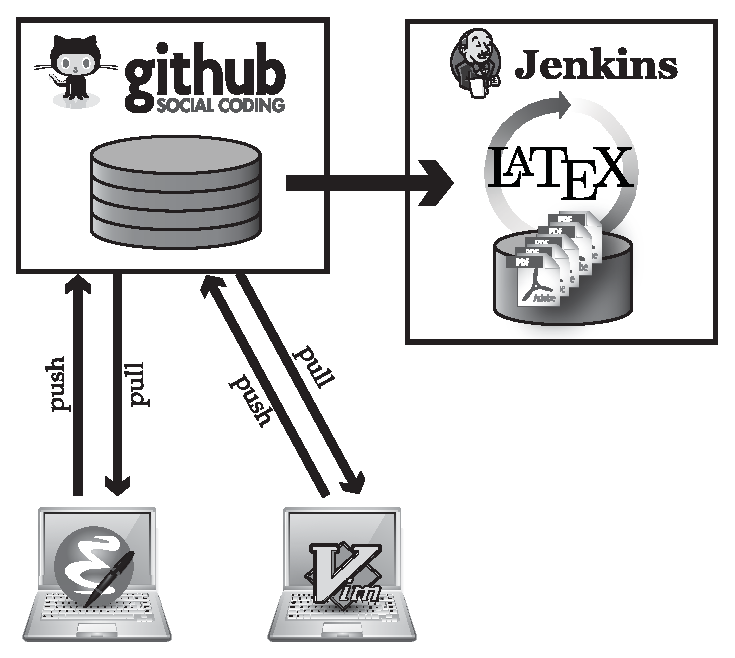
\includegraphics[width=8cm]{images/dbtimes-env.eps}
% \end{center}

\section{LaTeX}

文章執筆はLaTeXに限る。

% 文章ファイルの保存形式は,やはりプレインテキストでなければならない。最近
% はWordも構造化された文章を執筆するための機能が整いつつあるという。しかし
% ながら,我々はプログラマである。プログラマは,各自の研ぎ澄まされたテキス
% トエディタ環境を有している。即ち,執筆速度を最大化するためには,各々が最
% 大限能力を発揮できるテキストエディタ環境を利活用することが最善である。そ
% のためには,やはりプレインテキストでなければならない。

文章ファイルの保存形式は,やはりプレインテキストでなければならない。プログラマは各自の研ぎ澄まされたテキストエディタ環境を有している。即ち,執筆速度を最大化するためには,各々が最大限能力を発揮できるテキストエディタ環境を利活用することが最善である。そのためには,やはりプレインテキストでなければならない。

そして,我々プログラマは情報を構造化されていない状況に極度のストレスを覚える生き物である。ある程度以上の長さ,内容の高度さをもつ文章を執筆する場合には,図表や章・節の参照,文献管理,目次の作成,整合性のある文章スタイル調整など,文章全体が高度に構造化され,文章内の要素が有機的に結合されていなければならない。これを為すためには,高度かつ柔軟な組版システムを利用することが必要不可欠である。

やはり,文章執筆はLaTeXに限る。

本誌の組版には \TeX Live 2011 を用いている。文書のクラスには奥村先生の{\tt jsbook.cls} を利用しており,{\tt tombow} オプションを利用することでトンボ付きの出力を得ている。{\tt tombow}オプションを利用する際には,併せて{\tt papersize}オプションを利用しないと,文書のサイズとしてはトンボ無しで出力されてしまうので注意が必要である。

\section{GitHub}

文章執筆はGitHubに限る。

複数名で共同作業を行う場合,最近では Dropbox が用いられる場合が多い。Dropbox は便利である。一度導入してしまえば,誰でも簡単にファイルを即時に共有することができる。

しかし,我々はプログラマである。プログラマは変更履歴を重んじる生き物である。即ち,バージョン管理システムはプログラマにとって必須である。Dropboxにも履歴管理機能は存在するが,限定的でありインターフェースも非効率なものである。

また,プログラマは編集の競合に注意を払う生き物である。特に本誌のように締め切りのあるようなものの場合,締め切り直前には多数の編集が競合することが予想される。Dropbox では,競合の解決をシステマティックに行うことは不可能である。一方,バージョン管理システムはその基本機能として競合解決のシステマティックな方法を提供する。バージョン管理システムに高いリテラシを有する我々にとって,これを用いないことは有り得ない。

そして今日,GitHubはプログラマの共通基盤である。殆どのプログラマは,各々のSSH公開鍵をGitHubに登録済みである。即ち,GitHubをバージョン管理システムのホストとして用いることで,最小限の手間で共同作業基盤を構築可能である。

幸いなことに,私はGitHubのプライベートレポジトリを作成できるアカウントを保有している。そのため,原稿はクローズドな形で管理することが可能である。

やはり,文章執筆はGitHubに限る。

\section{継続的インテグレーション}

文章執筆は継続的インテグレーションに限る。

我々は重要な事実に目を向けなければならない。\LaTeX の基盤たる \TeX という言語は,単なるマークアップ言語にあらず。チューリング完全性を有する,完備なるプログラミング言語であり,\LaTeX による文章執筆とは即ちプログラミング行為であり,ソフトウェア開発にほかならないのである。

ソフトウェア開発において,今日最も重要視されている開発基盤の一つが継続的インテグレーションである。バージョン管理システムにコードがコミットされる度に,プログラムがビルドされ,テストコードが走り,常に最新の成果物が生成された状態が維持される。一度誤ったコードがコミットされた折には,そのことが開発者に直ちに通知され,更なる状況の悪化を食い止めるフィードバックループを形成する。

% また,\LaTeX による文章執筆における特有の問題として,最終成果物であるPDF
% ファイルに正しくフォントを埋め込むための環境構築には一定の手間を要すると
% いうことがある。執筆者全員が,あまねく必要なフォントをすべて保持し,適切
% に \LaTeX 環境を設定することは難しい。必要なフォントを持たない場合には,
% 代替フォントによって文章をプレビューする他にない。一方で,継続的インテグ
% レーションのためのビルドサーバにおいてこのような環境を構築しておけば,執
% 筆者全員が最終成果物を正しい形で確認することが可能である。

本誌の執筆においては,継続的インテグレーションシステムJenkinsを導入し,GitHubのコミットにフックしてPDFファイルの生成を行うことにより,即座に入稿可能な状態の原稿が常に確認可能な環境を構築した。

やはり,文章執筆は継続的インテグレーションに限る。
% -*- coding: utf-8 -*-

% TODO: 読点句読点の置換
% TODO: タイトル考える
\chapter{IRRのおはなし}
% * (アスタリスク)付きの \chapter* コマンドは原則不可とする

\begin{flushright}
 {\headfont yuyarin} % ペンネーム
\end{flushright}

インターネットにおけるドメイン間ルーティングでは,運用の利便性やセキュリティの面から経路情報を管理するデータベースが求められている.
そこで使われるのがルーティングポリシーを記述することを目的としたIRR(Internet Routing Registry)というシステムである.
本稿ではIPルーティングの基礎を簡単に述べた後に,ドメイン間ルーティングの運用と経路ハイジャックの問題について述べ,IRRをの仕組みと現状を紹介する.

この記事ではIP通信の基礎(IPアドレスとサブネット,パケット転送の仕組み)に関する知識を有していることを前提とすることをご了承頂きたい.


% TODO: セクション区切りを考える
\section{AS間ルーティングと経路フィルタ}

\subsection{経路交換とルーティング}

% 図を書く?
IPネットワークの役割は宛先のノードまでIPパケットを届けることであるが,
宛先に対してパケットを届けるためには,どのルータにパケットを転送すればよいかを知る必要がある.
パソコンなどのエンドホストは出口になっているルータ(デフォルト・ゲートウェイ)にパケットをすべて送ればよいが,途中のルータはそうはいかない.
そのためにはルータ間で自分の到達可能な宛先ネットワークの情報を交換する.
経路を他のルータに伝えることを\textgt{経路広告}と呼び,お互いが広告し合う事で\textgt{経路交換}が行われる.

経路交換を行い,集められた経路情報からパケットを送信する経路を決定することを\textgt{ルーティング}と呼び,そのためのプロトコルを\textgt{ルーティングプロトコル}と呼ぶ.
ルーティングによって選ばれた経路はベストパスと呼ばれる.

経路は大きく分けて,\textgt{宛先ネットワーク},\textgt{ネクストホップ},\textgt{メトリック}の3つの情報で構成される.
宛先ネットワークは192.0.2.128/25のようにprefixで表現される.
ネクストホップは宛先ネットワークにパケットを送るために次にパケットを転送するノードのアドレスである.
メトリックは宛先ネットワークに対して複数のネクストホップがあった場合にどのネクストホップを優先するかを決めるための値である.
この値の内容はルーティングプロトコルによって異なる.

\subsection{ASとドメイン間ルーティング}

% 図を書く?
1つの同じポリシーで運用されるネットワークの範囲を\textgt{ドメイン}と呼ぶ.
また,このドメインを\textgt{AS(Autonomous System, 自律システム)}と呼び,4 byteの一意な番号である\textgt{AS番号}によって区別される.
なのでインターネットはASという自律的なネットワークが相互に接続した「ネットワークのネットワーク」ということができる.

ASの内部で行われるルーティングを\textgt{ドメイン内ルーティング(Intra-domain Routing)}と呼ぶ.
ドメイン内ルーティングは各ASで好きなように行うことができる.
日本ではOSPF,北米ではIS-ISが主なルーティングプロトコルとして利用されている.

ASの間で行われるルーティングは\textgt{ドメイン間ルーティング(Inter-domain Routing)}と呼ぶ.
ドメイン間ルーティングは全世界のすべてのASで共通のルーティングプロトコルを利用しなければならず,現在はBGP4が利用されている.
ドメイン間ルーティングではドメイン内のルーティングは隠蔽されている.

ある経路について経路広告を行なっている大元のASのことをOrigin ASと呼ぶ.

\subsection{AS間の接続関係}

インターネットはASが相互接続してできたネットワークであるという話をしたが,すべてのASが対等に接続しているわけではない.
AS間の関係には大きく分けて上下関係のトランジット(transit)と対等な関係のピア(peer)の2つが存在する.
このASの強弱関係は接続しているASの数や知っている経路の数,つまり到達性の広さで決まってくる.

トランジットはお金を支払って他のASから接続性を買う関係である.「トランジットを買う」とも言う.
接続性を売る側を親ASやトランジッタ,買う側を子ASやカスタマーなどと呼ぶ.
トランジットでは流れるトラフィック量に応じてMbps単価で月額料金が課金されることが多い.

ほとんどのASはトランジットを上位のASから購入している.どこからもトランジットを買わない最上位のASはTier 1と呼ばれる.
現在14のASがTier 1とされており,日本の事業者ではNTT CommunicationsのAS2914が唯一のTier 1である.

一方でピアは強弱関係の近いAS同士が無償で経路交換を行う関係である.
一般に「ピアを張る」と表現されるが,BGPにおける隣接関係をピアと呼ぶため,トランジットの関係でも技術的には「ピアを張る」ので文脈に注意する必要がある.
もともとトランジットを通して行われていたトラフィック交換をピアによって直接行うことにより,従量課金であるトランジットの使用料を下げることができる.

\subsection{経路広告とトラフィックコントロール}

さて経路広告を行うと,その経路宛のパケットが流れこんでくる.
正確には対向ASのルータにおいてルーティングのプロセスでベストパスに選ばれればである.

経路広告をしてもらうと,その経路宛のパケットが対向ASのルータに吸い込まれる.
自分ASのルータでベストパスに選ばれた対向ルータに吸い込まれるが,自分のASのルータなので制御は簡単である.

必要なトラフィックは自分のASを通して流しても良いが,自分に全く関係のないトラフィックであれば,
たとえお金のかからないピアであっても流したくないし,ましてやお金のかかるトランジットには死んでも流したくない.
平たく言えばタダ乗り禁止である.トラフィックが増えるほど設備が必要になるからだ.

そういった経済的な動機によって,トラフィックをコントロールしなければならないのだが,基本原則は存在する.
トランジットでは,親ASは子ASの広告する経路を全世界に対して広告する責任があり,子ASは親ASからの経路をすべて受け入れる.
ピアでは,自分の子ASと自ASの経路を広告し,ピア先のASとその子ASの広告する経路を受け入れる.
このへんの詳しい話は非常に面白いところだけれども,今回の本題からは逸れるのでまたの機会に.

トラフィックをコントロールする方法はいくつか存在するが,AS間においてはまず経路を広告するかしないかの二択である.
メトリックなどの細かいパラメータは経路を広告すると決めてからの話である.

\subsection{経路フィルタ}

どの相手にどの経路を広告するか,どの相手からのどの経路広告を受け入れるか,それを制御するためにルータに経路フィルタを設定する.
そのため,自ASが新しく経路広告を行うときは隣接ASにそれを伝えてフィルタを開けてもらわなければいけいない.
これにはメールが使われていることが多いが,隣接ASが自ASの経路を広告している場合は,さらにその隣接ASにもフィルタを空けてもらう必要がある.
このようなケースはトランジットで起こりうるのだが,最上位のTier 1の労力は半端なものではない.
AS RankによればAS2914は全世界の約1/3の13,242の子ASを抱えて156,530のIPv4の経路を広告している.
人手のかかるメールなんかではやってられないので,経路情報をデータベース化して自動的にフィルタを生成して反映される仕組みが必要になってくる.

\section{資源管理と経路ハイジャック}

\subsection{AS番号とIPアドレスの関係}

インターネットは自律的なシステムではあるが,AS番号やIPアドレスなどの資源は重複利用が生じないように誰かが統一的に管理を行わなければならない.
こういった資源は階層的に組織されたInternet Registryによって管理されていて,
日本の場合では,最上位のIANA,アジア太平洋地域のAPNIC,日本国のJPNICのようにして階層的に資源が割り当てられている.
ちなみに欧州地域はRIPE,北米地域はARINで,日本におけるAPNICに相当する.
日本国内でAS番号やIPアドレスを取得する場合はJPNICを窓口として割り振りを受ける.

AS番号もIPアドレスもそれぞれが取得を申請した組織や個人に割り振られるため,AS番号とIPアドレスは資源管理上は直接の関係性を持っていない.
また,一つの組織が複数のASを運用することも多いし,他の組織の子ASにアドレスブロックを貸与することもあるため,
実際にどのASからどの経路が広告されるかは,広告されてみないとわからない.
もちろんネットワークの運用者は自分のASから広告する経路を知っているが,他のASのことはわからない.

\subsection{経路ハイジャック}

JPNICのような組織からまだ割り振りを受けていないアドレスブロックや,
他の組織が取得しているアドレスブロックを勝手に広告することは技術的には可能である.
単純にルータにそういう設定を入れればいいだけで,免許のようなものはいらない.
こういう事例を経路ハイジャックと呼ぶ.

前章で経路を流すとトラフィックが流れることを説明した通り,経路ハイジャックを受けると,
本来自分のASに流れるはずだったトラフィックが他のASに流れてしまう.
パケットが到達不能で破棄される可能性や,盗聴・改竄の恐れもある.

経路ハイジャックは頻繁に起きていて,そのほとんどはアドレスの打ち間違いやAS外に出さない経路を漏らしてしまうなどの設定ミスである.
大規模な事件としてはパキスタンテレコムがYouTubeの経路をハイジャックしてしまい,YouTubeにアクセス不能になった事件などが挙げられる.
この事件ではパキスタン国内でYouTubeへのアクセスを遮断するために偽の経路情報を流してトラフィックを吸い込もうとしたところ
設定ミスで偽の経路情報をAS外部に漏らしてしまったのが原因だと言われている.

こうした経路ハイジャックが行われた際に,すぐに気づくことが出来る仕組みが必要になる.
経路ハイジャックかどうかを調べるためには,その経路のOrigin ASが妥当であるかを見ればいいのだが,
前述のとおりASとIPアドレスの対応表なんてものはないため,調べることはできない.

根本的な解決として署名付きの経路を流すBGPsecなどが提案されているが,
ひとまずの運用的な対処として,Origin ASと経路の関係性の情報を持ったデータベースを作成して,
それとBGPで実際に流れている経路を比較することで,ハイジャックを検知する取り組みが行われている.
そのためには当然,正確なOrigin ASと経路の関係性の情報を持ったデータベースが必要になる.

\section{IRR}

\subsection{IRRとは何か}

さて,ここまで経路フィルタの自動生成という運用上の問題と経路ハイジャックの検知という2つの目的から,
経路に関連する情報を持ったデータベースが必要になっているという話をした.
そこで登場するのがIRR(Internet Routing Registry)である.
名前の通り,インターネットのルーティング情報を登録するシステムで,
もともとは高度なルーティングポリシーを記述でき,その運用者の情報なども管理できるものである.

歴史を少し述べると,IRRは,1980年代のNSFNetの時代にコンフィグを自動生成するための,高レベルなルーティングポリシーを記述するためのデータベース(PRDB)から由来している.
その後,1989年にRIPEの最初のミーティングが行われ,1994年にRIPE-181という文書で現在使われているオブジェクトクラスベースの構造の概念が導入され,1995年にIETFにてRFC1786として標準化さた.
最終的に1999年にRFC2622 Routing Policy Specification Language (RPSL)として標準化されRFC4012でIPv6用の拡張が行われ現在に至っている.

IRRではwhoisをプロトコルに使っているためwhoisコマンドを用いて利用することができる.
実装はRIPE NCCのRIPE DB ServerとMeritのIRRdの2つがメジャーである.

\begin{quote}
\begin{verbatim}
$ whois -h jpirr.nic.ad.jp AS4713
\end{verbatim}
\end{quote}

\newenvironment{minilinespace}{
\baselineskip = 4mm
}

\begin{tabular}{l}
\begin{itembox}[c]{aut-numオブジェクト}
\begin{quote}
\begin{minilinespace}
\begin{verbatim}
% whois -h whois.radb.net AS2500 
aut-num: AS2500
as-name: WIDE
descr:   WIDE Project in Japan
admin-c: JM46-AP
tech-c:  AK27-AP
import:  from AS-NSPIXP2
           action pref=100;
           accept ANY
import:  from AS2501
           action pref=100;
           accept AS2501 AS7531                     
(snip)
export:  to AS-NSPIXP2 announce AS112 AS2500 AS2501 (snip) AS55384
export:  to AS2504 announce ANY and NOT AS7660      
(snip)
notify:  two@wide.ad.jp
mnt-by:  MAINT-AS2500
changed: kato@wide.ad.jp 20121024
source:  RADB
\end{verbatim}
\end{minilinespace}
\end{quote}
\end{itembox}
\\
\begin{itembox}[c]{routeオブジェクト}
\begin{quote}
\begin{minilinespace}
\begin{verbatim}
% whois -h whois.radb.net 1.1.1.1
route:   1.1.1.0/24
descr:   Google
origin:  AS15169
notify:  radb-contact@google.com
mnt-by:  MAINT-AS15169
changed: radb-contact@google.com 20121119
source:  RADB
\end{verbatim}
\end{minilinespace}
\end{quote}
\end{itembox}
\\
\begin{itembox}[c]{as-setオブジェクト}
\begin{quote}
\begin{minilinespace}
\begin{verbatim}
% whois -h jpirr.nic.ad.jp AS-OCN
as-set:  AS-OCN
descr:   ASes advertised by OCN
members: AS4713,
         AS290,   AS1628,  AS2499,  AS2506,  AS2509,
         AS2515,  AS2518,  AS2526,  AS4680,  AS4683,
         (55 lines snipped)
         AS131154, AS131154, AS131155, AS132095, AS132119
admin-c: Ichiro Mizukoshi
tech-c:  Tomoya Yoshida
notify:  admin@ocn.ad.jp
mnt-by:  MAINT-AS4713
changed: admin@ocn.ad.jp 20121206
source:  JPIRR
\end{verbatim}
\end{minilinespace}
\end{quote}
\end{itembox}

\end{tabular}

\subsection{IRRの構造}

IRRにはいくつかの種類のクラスが定義されていて,それらをオブジェクトとして登録していくことで成り立っている.
RFC2622/4012では,
route, route6, aut-num, as-set, route-set filter-set rtr-set peering-set inet-rtr, mntner, role, person
といったクラスが定義されている.このうち今回は特によく利用されているaut-num, route, as-setについて紹介する.
百聞は一見にしかずなので登録されているデータを見て頂きたい.

\subsubsection{aut-numクラス}
aut-numクラスはASを表現したクラスでASという接頭辞の後にAS番号を続けたものをキーに使う.
大体の属性値は見ていただければわかると思うが,特筆したいのが,export/import属性である.
この属性には肝心要のルーティングポリシーを記述することができる.
importの例では,AS-NSPIXP2(これは後述のAS-SETオブジェクト)に含まれるASから広告されるに対して,
経路のpreferenceを100にしながらすべての経路を受け入れるというポリシーを記述している.
一方でAS2501からの経路に対してはAS2501とAS7531の2つのASがOriginである経路しか受け入れない.
exportの例ではAS2504に対してAS7660を除くすべての経路を広告するというポリシーを記述している.

この例はAS2500のWIDE Projectという日本の研究機関のASのものであるが,
先に述べたようにASの接続関係は接続性の売り買いの話につながるため,
ポリシーがオープンなコンテンツプロバイダや研究機関を除いた商用のISPなどで,
ここまで細かく記述されていることは滅多に見かけない.

\subsubsection{routeクラス}
routeクラスは経路情報を表現したクラスで,広告されるプレフィックスをroute属性に使う.
IPv6の経路はroute6クラスで表現される.
origin属性にはその経路を広告するASのaut-numオブジェクトが書かれていて,routeとoriginを合わせてこのオブジェクトのキーとしている.
そのため1つの経路に対して複数のoriginが存在することもある.
運用上複数のOrigin ASから同一の経路を広告する可能性があるため,そのようになっている.

\subsubsection{as-setクラス}
as-setクラスはaut-numオブジェクトの集合体を表現したクラスで,AS-という接頭辞の後に名称を続けたものをキーに使う.
例はAS-OCNというNTT CommunicationsのOCN(AS4713)のas-setである.
このASは国内のトランジット事業者でもあるので多くの子ASを抱えており,その経路を上位のトランジットに対して広告する必要がある.
その際にAS4713の子ASが誰であるかを上位ASはいちいち気にしたくないので,as-setとしてまとめて教えてあげている.

\subsubsection{mnt-by属性とsource属性}
これらのクラスに共通して存在する属性の中にmnt-by属性とsource属性がある.
mnt-by属性はそのオブジェクトを管理している組織を示す属性で,mntnerクラスのオブジェクトが登録される.
mntnrクラスのオブジェクトにはパスワードが設定できるため,mnt-by属性を指定することで他者からのデータの上書きを防ぐことができる.
source属性はそのオブジェクトがどのIRRに登録されたものかを示している.
後述するがIRRは複数の組織で独立して運用されていて,それらの間でデータを同期している.
問い合わせを行うIRRホストと,オリジナルのオブジェクトが登録されているIRRホストは別になるため,この属性が必要になる.

\subsection{IRRの運用}

IRRは世界の30以上の組織でそれぞれ運用されている.
APNICやJPNIC,RIPEなどのInternet Registryが運用するもの,NTT CommunicationsやLevel3などのISPが運用するもの,Meritなど研究機関が運用するものに分類することができる.
日本から使う場合はJPNICのJPIRR,MeritのRADB(Routing Assets Database),NTT CommunicationsのNTTCOMが有名である.

これらのIRRはデータベースを他のIRRと同期しているが,組織の関係によっては同期していないこともある.
例えば研究機関であるMeritの運用するRADBはほとんどのIRRのミラーを行なっている.
NTTCOMはJPNICのJPIRRをミラーしているが,JPIRRはNTTCOMをミラーしていない.
これは公的機関が一営利企業のミラーを行うということに対する大人の事情でそうなっている.

\subsection{IRRが必要とされる場面}

IRRは任意加入のデータベースだが,利用を迫られる時がある.
基本的には経路フィルタの自動生成を行うためにIRRが使われる.

例えばNTTCOMやLEVEL3のようなTier1トランジット(ISPのためのISP)では経路フィルタ適用などの運用を簡略化するために,
顧客に対して自身のIRRに経路情報を登録することを求めている\footnote{http://www.us.ntt.net/support/policy/rr.cfm}.
また同様の理由で他のASに対してピアを張るための条件としてIRRの登録を求めるASも存在する.
他にもIX(Internet Exchange)でroute serverを使ってmulti lateral peeringを行う際の経路フィルタの登録などにも利用される.

フィルタの生成の他には経路情報からコンタクトパーソンを見つけるためや,
障害時のトポロジー把握などに使われる.

\subsection{IRRの歩き方}

ではそろそろ手を動かしたくなって疼いてきた頃だと思うので,一般のご家庭でよく使われるIRRの使い方を紹介しよう.

origin ASを指定して経路の一覧を取得するときは!gを使う.
UNIXの場合は!を\verb+\+でエスケープする必要がある.
メモリ管理が必要な古のプログラムからでも読みやすいように整形されて表示され,Aはデータの長さ,Cは終了を意味している.

\begin{quote}
\begin{minilinespace}
\begin{verbatim}
% whois -m \!gAS7521
A116
210.173.160.0/19 210.173.176.0/24 210.173.178.0/25 218.100.45.0/24 (snip)
C
\end{verbatim}
\end{minilinespace}
\end{quote}

AS-SETをASの一覧に展開したいときは!iオプションを使う.AS-SETの中にAS-SETが含まれるような場合は,1をつけてAS-SETの再帰展開を行う.

\begin{quote}
\begin{minilinespace}
\begin{verbatim}
% whois -m \!iAS-GOOGLE,1 
A126
AS11344 AS13949 AS1424 AS15169 AS19425 AS22577 AS26910 AS36040 (snip)
C
\end{verbatim}
\end{minilinespace}
\end{quote}

AS7521がメンテナになっているオブジェクトを列挙する.だいたいこのあとに属性でgrepをかける.

\begin{quote}
\begin{minilinespace}
\begin{verbatim}
% whois -m \!oMAINT-AS7521 
A10130
route:      210.173.160.0/19
descr:      INTERNET MULTIFEED CO.
(snip)
source:     JPIRR
C
\end{verbatim}
\end{minilinespace}
\end{quote}

AS7521の情報でsourceがJPIRRのものだけを選択する.sourceによっては情報が間違っていたりすることがあるので,
情報の信頼性の高いsourceを指定したくなる場合がある.
ダブルクオーテーションで囲ってwhoisのオプションに間違われないようにする.

\begin{quote}
\begin{minilinespace}
\begin{verbatim}
% whois -h jpirr.nic.ad.jp -- "-s JPIRR AS7521"
aut-num:    AS7521
as-name:    MFEED
(snip)
source:     JPIRR
\end{verbatim}
\end{minilinespace}
\end{quote}

\subsection{もっと楽しいIRRの使い方}

ISC(Internet Systems Consortium)が開発しているIRRToolSet\footnote{http://www.isc.org/software/irrtoolset}を使うことでもっと快適なIRR生活を送ることができる.

pevalはIRR用にwhoisをもっと簡単にしたものである.as-ocn and as-iijのような記述をすればOCNとIIJの両方から広告されているプレフィックスの一覧
(OCNとIIJでマルチホーム接続しているASの経路)を取得することができる.

\begin{quote}
\begin{minilinespace}
\begin{verbatim}
peval "as-ocn"
({223.223.164.0/24, 223.223.165.0/24, 223.223.166.0/24, ... })
peval "as-ocn and as-iij"
src/peval/peval "as-ocn and as-iij"
({223.223.160.0/22, 223.223.0.0/17, 223.29.244.0/22, ...})
\end{verbatim}
\end{minilinespace}
\end{quote}

RtConfigはCiscoやJuniperのルータ用のフィルタやstatic routeを生成することができるツールである.

\begin{quote}
\begin{minilinespace}
\begin{verbatim}
% rtconfig -cisco_use_prefix_lists
rtconfig> @RtConfig access_list filter AS15169
!
no ip prefix-list pl100
ip prefix-list pl100 permit 1.0.0.0/24
ip prefix-list pl100 permit 1.1.1.0/24
ip prefix-list pl100 permit 1.2.3.0/24
ip prefix-list pl100 permit 8.8.4.0/24
ip prefix-list pl100 permit 8.8.8.0/24
ip prefix-list pl100 permit 8.34.208.0/20 ge 21 le 21
ip prefix-list pl100 permit 8.34.208.0/20 ge 23 le 24
(snip)
ip prefix-list pl100 deny 0.0.0.0/0 le 32

% rtconfig -config junos
rtconfig> @RtConfig access_list filter AS290
policy-statement prefix-list-100 {
  term prefixes {
    from {
      route-filter 45.1.0.0/16 exact accept;
      route-filter 130.128.0.0/15 prefix-length-range /16-/16 accept;
      route-filter 202.17.221.0/24 exact accept;
    }
  }
  term catch-rest {
    then reject;
  }
}
\end{verbatim}
\end{minilinespace}
\end{quote}

\section{IRRの問題}



% -*- coding: utf-8 -*-

\chapter{パターン認識の「構造と力」---逃走論を超えて---}
% * (アスタリスク)付きの \chapter* コマンドは原則不可とする

\begin{flushright}
 {\headfont 早水 桃子}% ペンネーム
\end{flushright}

\begin{spacing}{0.7}
\normalsize{
\noindent
標題(と傍題\footnote{傍題もやはり浅田彰の『逃走論---スキゾ・キッズの冒険』に因む。})が示すように、本稿は『構造と力---記号論を超えて』へのオマージュとして書かれている。質の悪いパロディと言っておくのが分相応かもしれないが、いずれにせよ1985年生まれの私が1983年の浅田彰の「力」に今も引き摺られているということは、告白するまでもなさそうだ。もちろん本稿は出典が記されている部分を除き、私という一個人の私見を述べたものに過ぎない。それは各分野の専門家の意見と一致するとは当然限らないし、またそれを期待したわけでもない。

\noindent
まずは歴史の中から一世を風靡した学問の例を引っ張り出し、この場違いな試論のスタンスを明らかにすることから始めたい(第1節)。そのスタンスでデータマイニングというものを批判的に考察する(第2節)。データ解析以外の領域における機械学習の姿を少しだけ眺めてから(第3章)、最先端の医学研究(第4節)と日常的な医療現場(第5節)に進んでいく。そこで直面するのは人間の脳は壊れるという現実であり、一貫した問題意識の中で大規模データベース・機械学習・古典統計学の諸概念を捉え直す。その先にあるのはデータベース・機械学習・古典統計学という枠組みを否定したときに何が残るのかという問いであり(第6節)、本稿の目論見はこの問いに対する答えの一つを提示することにある(第7・8節)。
}
\end{spacing}
 
\section{来し方行く末}
\subsection{無識なる者たち}
『解体新書』は江戸時代の医師たちの試行錯誤によって『ターヘル・アナトミア』というオランダ語の解剖学書から翻訳され、1774年に出版された歴史的書物である。まだオランダ語の辞書すらなかった時代であることを考えると、本文・図表合わせて五冊から成る医学書をわずか数年で翻訳・出版したというだけで大変な偉業である。しかしこの本の偉大さは、当時鎖国政策をとっていた日本に初めて西洋の医学知識を伝道し、それまでの日本の常識を覆したところにある。
『解体新書』以前の日本においては解剖はほとんど行われていなかったため、人体は「五臓六腑」という東洋医学の概念によって捉えられていた。今でこそ我々は人体を色々な臓器の解剖学的な構造と生理学的な機能が作るシステムとして捉えているが、人体の構造を捉える解剖学という枠組みを日本に初めてもたらしたのは、『解体新書』に他ならないのである。

『解体新書』は医学にとどまらず、ヨーロッパで発展した様々な学問から新しい知識や技術を吸収するという「蘭学(洋学)」ブームの契機になり、近代日本科学史に金字塔を打ち立てることとなった。
しかし、『解体新書』の翻訳者の一人である杉田玄白は、彼が85歳で亡くなる2年前に著した『蘭学事始』(1815年)という回想録の冒頭において、このブームを少々醒めた目で眺めている。
%蘭学草創期の出来事を正しく伝えるために、85歳で亡くなる2年前の1815年に『蘭学事始』という回想録を著し、その冒頭でこのように述べている。

\begin{quote}
\ruby{今}{きん}\ruby{時}{じ}、世間に蘭学といふ事専ら\ruby{行}{おこな}はれ、志を立つる人は\ruby{篤}{あつ}く学び、無識なる者は\ruby{漫}{みだ}りにこれを誇張す。
\end{quote}

唐突に、「蘭学」を「機械学習」に置き換えるという悪ふざけを試みる。この操作のバカバカしさとは裏腹に、「無識なる者」が我々に冷たく突き刺さる言葉に化ける。
%バズワードに煽られる烏合の衆を「無識なる者」と批評することこそ、「無識なる者」という言葉に冷や汗をかいていることの裏返しなのではないだろうか。
人体を切り刻んで臓器や組織ごとに描写する解剖学アトラスの構造は、数多くの理論や方法を網羅的に記述することのようでもある。この文脈で『解体新書』に重なるのは、やはり『パターン認識と機械学習』\footnote{本稿の読者には説明不要であろうが、``Pattern Recognition and Machine Learning''(C. Bishop)を邦訳した教科書である。ちなみに「ベイズ理論による統計的予測」という副題が添えられている。}だろう。自分は「無識なる者」の外側にいるのだと信じようとするほど、内側に引き摺り込まれる------そんな気分にさせられる。


「情報爆発」や「ビッグデータ」へのソリューションが声高に語られる2012年の状況は、
John Naisbittが ``We are drowning in information but starved for knowledge.''(我々は情報の海に溺れ、知識に飢えている)\footnote{John Naisbitt ``Megatrends''(1982)より引用。}と評した1982年から変わったとはお世辞にも言えないはずだ。そして残念ながら杉田玄白が苦言を呈した1815年からも、多分大きな変化はないのだろう。

新しいものに魅力を見出すこと自体は、むろん健全な知的好奇心である。いただけないのは「無識なる者」が多数派になることである。それは最先端の花形的研究分野の活気ではなくて、ゴールドラッシュ\footnote{金が採掘された場所に一攫千金を目論む採掘者が殺到すること。1848年にカリフォルニアの川で砂金が発見されたことによるカリフォルニア・ゴールドラッシュが有名であるが、金の鉱脈が見つかるたびに世界各地で幾度となく繰り返し見られる現象である。}を彷彿とさせる熱病と呼ぶべきものだからだ。

\subsection{メルトダウンするブームと心中しないために}
もっとも、人並みの繊細さを持ち合わせている人間であればその熱気にのぼせて付和雷同してはいられないだろう。現在のデータサイエンスをとりまく熱気は単なる空騒ぎに浪費されるかもしれないし、これまでに提案されてきた数々の理論や技法は、現実の問題解決に対する有用性や意義が不明瞭なまま忘れ去られ、それを実装したコードも無用の長物となるかもしれない。データ解析に求められるソフトウェア・ハードウェアに投資しても望む結果が何も得られなかったとしたら、ユーザーの少々無理のある過剰な期待はやがて失望に変わり、それが集団的な絶望へ変わる時にブームは終焉を迎える。最悪の場合は学問分野そのものまで廃れていってしまうかもしれない。

そして蘭学は亡骸になった。一世を風靡し、蘭方と漢方の深刻な医学的対立を招き、蘭書翻訳取締令により思想弾圧の憂き目を見ることになった。19世紀の英国に目を向けてみれば、もっとストレートな例を見出だせるだろう。
産業革命は機械による自動化・作業効率化をもたらした一方で、失業を恐れた労働者集団に機械破壊という行動をとらせてしまい\footnote{この機械打ち壊し運動(ラッダイト運動)になぞらえて、雇用を不安定にするIT化・自動化に反対する思想はネオ・ラッダイトと呼ばれている。}、産業廃棄物という未解決の問題を山積みにしてしまった。どれほど優れたものだと言われてきたとしても、人間はそれを排除することもあるし、新たな問題の元凶とみなすこともある。持て囃されているものが、定着するとは限らない。そんなことはもう幾度となく思い知らされてきたはずだ。
%人間が生み出した新しいものを活かすのも人間であり、殺すのも人間であるということを心に留めておきたい。

とはいえ、「無識なる者」を見下して優越に浸るのは、自意識過剰な批評家だけでいい。ならば時代の潮流に乗るために必要なものとは何なのだろうか。
------もしも思考が淀みかけたなら、今すぐキューを手に取って、ビリヤードの練習がてらブレイクショットを打とう。キューボールは「自ら『濁れる世』の只中をうろつき、危険に身をさらしつつ、しかも、批判的な姿勢を崩さぬこと」。それは「対象と深くかかわり全面的に没入すると同時に、対照を容赦なく突き放し切って捨てること」で、まさしく「シラケつつノリ、ノリつつシラケること、これである」\footnote{『構造と力』の序文から立て続けに引用。}。

スタート地点における我々のスタンスが決まったところで肝に銘じておくべきことがある。理論や技法がどれほど高度なものであろうとも、現実世界では人間の目的を叶える手段に過ぎないということである。目的を設定するのも人間であり、道具を使うのも人間である。だから道具の格付けに一喜一憂するとか道具を使うこと自体が目的化するというのは狂信的と言わねばなるまい。道具を「学習」したら終わりという態度だって、望ましいはずがない。「急いで狭苦しい枠組を作り、その中に閉じ込もってチマチマと空白を埋めていくという、一見勤勉そのものの『学習』態度、その実、これ以上の怠惰はない」わけである。目的の見えない虚しい学習は義務教育で卒業しよう。さもなくば人工知能に笑われる。

データベースからの知識発見という舞台を観客として眺めていると、大規模データベース・機械学習・統計学という役者たちの華やかさに惑わされそうになる。「道具」たちは何ができて、何ができないのか。互いにどのように関わり、どこでどのように応用されるべきなのか。それが混沌を極めているとしたら、おそらく何かとてつもなく単純なことを見落としている。それは目的が存在しなければ道具箱もショーケースになってしまう、ということだ。カオスの中から浮かび上がるストーリーは、人間の問題意識や目的なしに始まるはずがなく、そして終わるはずもない。

\section{データマイニング再考}
まずはJerome H. Friedmanの``Data mining and Statistics: What's the connection?''(1997)を下敷きにして、データマイニングとは何であるのかを掘り下げてみよう。

\subsection{データマイニングとデータベース}
データから知識を得ようとすること自体に目新しさはないはずだ。では、何が今頃になってデータマイニング「特需」をもたらしたのだろうか。この問いかけに答える鍵の一つは、データベースマネジメントシステム(DBMS)の変遷である。
%Imielinski(1995年)

かつてのDBMSにおいては、銀行のATMで利用されているようなオンライントランザクション処理(OLTP)と呼ばれる情報処理が主流であった。つまり、DBMSに求められていたのはデータを貯蔵し、多くのユーザーからの小規模なデータアクセスを伴う定型クエリーを高速に処理するという能力だった。
%http://otndnld.oracle.co.jp/deploy/performance/pdf/Oracle8i-tuning2.pdf
しかしデータベースに蓄積されたデータを様々な切り口で分析したい人々が
データベースに意思決定支援を求めるにつれて、新しい情報処理が注目を集めるようになった。それが
オンライン分析処理(OLAP)である。

OLAPによってユーザーは対話式の試行錯誤を繰り返して、データウェアハウスに格納された膨大なデータを集計したり、あるいは多次元的に分析したりといったことができるようになった。
一見するとこれはデータマイニングツールの原型のように見えるかもしれない。しかし、OLAPによるデータ解析によってデータウェアハウスと「対話」できるのは、的確な仮説を考え続けるような不断の洞察力とクエリーを書き続ける技術力(および時間と体力)を持ち合わせた選ばれし人間だけである。データに潜むパターンやモデルの叩き台を自動的に見つけてくれるものではないし、ビジネスの場における迅速な意思決定に向いているものでもない。だからこれは
データマイニングツールの原型と言うよりはむしろ、人々がデータマイニングツールを求める素地を作ったと考えたほうが良いだろう。
%大規模なデータからパターンを見出す試行錯誤のプロセスが人間の手を煩わせずに実現するならばそれが効率的であるし、data analysis for everyoneみたいなものへの需要は高まっていった。

\subsection{プロパガンダとしてのデータマイニング}
データマイニングもまた他のバズワードの例にもれず定義が曖昧な言葉だが、色々な定義をまとめるとしたら「
複雑で膨大なデータ集合の中に埋もれていて人間の力では見いだせないような有益な知識をコンピューターの力でデータベースの中から探索的に発見し、ビジネスにおける意思決定に役立てるような色々な手法(またはそれらを使ったプロセス)」というところであろう。実際のデータ解析にはIBM Intelligent miner、SAS Enterprise Miner、SPSS Clementineなどの汎用データマイニングツールが使われることが多い。

Knowledge Discovery in Databasesというデータマイニングの目論見は壮大なものである。しかし、
%データから新たな知見を得ようとする試みは全然斬新なものではない。
ユーザーが小難しいデータベースの構造やデータ解析の中身を知らなくてもデータベースに格納されたデータにアクセスすることを可能にし、それを分析したり視覚化したりしてくれるデータマイニングツールというものは
誰のためのものなのだろう。
「データ自身に語らせる」といえば聞こえは良いが、ビジネス戦略のヒントとなるような知識を囁くかどうかは別の話であるし、そんな都合の好い話はあまり聞かない。Friedmanが指摘するように、汎用データマイニングツールは非常に高額な商用ソフトウェアであり、導入するとなれば当然相応の高価なハードウェアやストレージも要求されることになる。その意味で、データマイニングはもはや金脈を掘り当てようとする宝探しのような試みというより、むしろデータマイニングと聞いてソフトウェアやハードウェアに投資してくれるような、データを持て余している企業の意思決定者や潜在的データマイナーを発掘するための商業的プロパガンダと化しているところがある。

\subsection{データマイニングと統計解析の違い}
Friedmanは汎用データマイニングツールが提供する主要な手法の数々を
%\footnote{Decision tree induction・rule induction・nearest neighbors・clustering・association rules・feature extraction・visualisation、neural networks・graphical models(Bayesian belief networks)・遺伝的アルゴリズム・SOM(自己組織化マップ)・neuro-fuzzy systemsと}
を列挙し
%\footnote{Friedmanは定番手法としてdecision tree induction(C4.5, CART, CHAID)・rule induction(AQ, CN2, Reconなど)・nearest neighbors(事例ベース推論)・clustering methods(data segmentation)・association rules(market basket analysis)・feature extraction・visualizationを挙げ、その他の手法としてneural networks・bayesian belief networks(graphical models)・genetic algorithms・self-organizing maps(SOM)・neuro-fuzzy systemsを挙げている。}
、多くのデータマイニングツールにおいて
仮説検定や判別分析など、統計学者にとって見慣れた手法は
殆ど無視されていると評している。一言で「データを解析する」といっても、データマイニングと統計解析は目的も手段も大きく異なるものであり、両者を混同してはならない。

統計学的なデータ解析は、「データ自身に語らせる」という大らかなものではない。
それは「実験が終わった後に統計学者にコンサルトするのは、死後に解剖を依頼するようなもので、統計学者はその実験の死因を教えることぐらいしかできない」というRonald Fisherの格言にも端的に表れている。
統計学者にとってはデータは綿密な実験デザインに基づいて注意深く収集され、吟味されるべきものであり、
鉱山のように元々そこにあるものではないのだ。

それに、データを説明するための仮説やモデルがなければ仮説検定もモデル選択\footnote{モデルのパラメータを最尤推定する「モデル推定」とともに、どのモデルを選ぶべきかという「モデル選択」は統計学・機械学習においては最も重要なテーマの一つである。AICやBICといった情報量規準が有名だがクロスバリデーションもよく使われる。}も始めようがない。良質なデータと洗練されたモデルこそデータ解析の要なのである。モデルが正しければ良い結果を出し、正しくなければ悪い結果を出すのがアルゴリズム(計算手法)のあるべき姿なのだから、解析結果の善し悪しはアルゴリズムではなくモデルが決めていると考えるのが筋である\footnote{本稿執筆時にインターネット上で配信されていた伊庭幸人氏(統計数理研究所)の「マルコフ連鎖モンテカルロ法の基礎」という講義の中でもモデル・統計手法・アルゴリズムの違いが強調されていた。}。

これに対しデータマイニングは、良く言えば従来の統計学が扱えないような整理されていない大規模データを何とか使える形にし、色々な切り口で分析して意思決定のヒントになる知識を見出そうとする果敢な取り組みである。悪く言えば産業廃棄物のような膨大なデータの山をゴミだと認めるわけにいかないからといって往生際悪くデータのフォーマットを整え、クレンジング\footnote{データの誤りや重複を洗い出し、使えるデータにするという泥臭い(しかし最も重要な!)プロセス。}を施して場当たり的に試行錯誤しながら有象無象の仮説やモデルの叩き台をあれこれ捻り出すという作業でもある。

いずれにせよデータマイニングは統計学とは全く異なる思想を持つものであり、仮説やモデルなしに鉱山の中を探索するデータマイニングにおいてよく登場する手法が、統計学の手法と異なるのは驚くべきことではないということが分かる。データマイニングが語られる文脈においてはテクニックやアルゴリズムありきの話になりがちであるのも、当然の成り行きなのかもしれない。

\subsection{データマイニングの意義}
しかしながら
%データマイニングに失望したり、ベンダーやコンサルティングファームに対して猜疑的になったり、
データマイニングの努力は水泡に帰するのかと悲観する必要はないし、それは本稿における我々のスタンスに反するはずだ。そこでの努力を無にしないためにできることがある、と考える程度の希望は持っていたい。

データマイニングに対して批判的になるのをここで一旦やめてみよう。少し楽観的になれば、データマイニングの功績が色々と浮かび上がるに違いない。従来の統計学では難しいような大規模で複雑なデータの解析も、プラクティカルな前処理の方法論も、複雑なデータの可視化による迅速な意思決定支援も、データマイニングなしには語れない。様々なテクニックを集めたツールとデータ解析の専門家だけでは解析結果が荒唐無稽なものになりがちだったが、それはデータマイニングは役立たないと切り捨てる理由にはならないはずだ。むしろデータ解析には現場の知識を持った専門家の関与が必須であるということを実証したといっていい。その教訓を\ruby{採掘}{マイニング}できなければ、ちょっとお粗末である。

データマイニングの商業的な側面ばかりを強調したが、大規模データベースを持っているのは企業だけではない。
後述するが、公開されている大規模なデータベースも色々と存在する。
そういうデータベースから知識を発見する試みにおいてデータマイニングは単なる商業的なプロパガンダに堕したものではなく、真理の探究を目指す学術研究において仮説やモデルのプロトタイプを見つける手段となったり、蓄積されたデータから合理的に最適な政策を決定するという国家や国際社会の意思決定を支援するためのツールとなり得る。

データマイニングは、クラスタリングや決定木学習に代表されるように、多様なパターン認識・機械学習の理論的な枠組みを現実の大規模データに応用してきた。そうした理論と現実の橋渡しをする取り組みは軽視されてはならないし、その価値は商業的な実用性や理論的な厳密さや一般性だけで評価されるべきではない。そうでなければデータマイニングバブル崩壊とともに、データベースから知識を発見することの重要性も失われかねないからだ。

\section{データベースの外側}
データ解析のことばかり考えていると、統計学もパターン認識も機械学習もデータベースを掘り起こす道具にしか見えなくなるかもしれない。このまま先へ進む前に、ほんの少しだけデータベースの外側に目を向けてみる。
\subsection{医療機器}
統計学や機械学習で登場するアルゴリズムの幾つかは、医療の現場で人々の健康な生活や生命を支えている計算手法と言っても過言ではない。医用画像を得るためには画像再構成という重要なプロセスがあり、そこではバックプロパゲーションやEMアルゴリズムといった機械学習・統計学でよく知られる手法が一般的に用いられている。
また、病気の検査のためだけでなく、
がんの放射線治療においてはモンテカルロ法が古くから線量分布推定に用いられ、
今もなお放射線治療計画に必須の計算手法であり続けている。

\subsection{神経科学}
もともと機械学習は人工知能研究の一分野であることから分かるように、理論神経科学と深く関係しており、その理論的な枠組みそのものが、人間の脳のメカニズムや、社会における人間の行動などを理解する一助となり得るものである。パーセプトロンは古くから小脳のモデルとして知られ、人間の運動学習の神経基盤を理論的にも実験的にも明らかにし、ロボットの運動制御という工学的な応用にもつながることとなった代表的な例である。
もう少し最近の例としては強化学習(特にTD学習)によるモデルがあり、これは大脳基底核の計算モデルとして注目されている。ドーパミンニューロンが報酬予測誤差によって強化学習を行っているという仮説が提唱され、報酬に基づく人間の意思決定の神経基盤が理論的にも実験的にも精力的に研究されている。こうした研究はパーキンソン病という大脳基底核が侵される神経変性疾患や、薬物・ギャンブル等への依存症などにも密接に関連している。

氷山の一角を一瞥しただけでも、これまでとは違った
統計学や機械学習の顔を垣間見ることができる。
とりわけ人間の脳につながる研究は興味深くて実際に有益でもある。しかしロマンティックな物語は別の機会に譲り、もう少しリアルで差し迫った話をしよう。

\section{認知症の研究:大規模データベースと機械学習の応用}
%日本人の平均寿命は世界の先進国の中でもトップクラスであり、それは高度に発達した現代の医学と、充実した医療サービスを誰でも受けることができるようにするための国民皆保険制度の賜物である。しかし
周知の通り、日本を筆頭に世界各国(特に先進国)で高齢化が社会問題化している。認知症患者は増え続けており、医療費の増加を通じて国の財政を圧迫し、若い世代にも大きな負担となっている。

認知症は社会だけでなく個人にとっても人生を脅かす問題である。
厚生労働省によれば日本では現在既に65歳以上の高齢者のうち約10\%が認知症であると見積もられており、しかも今後さらに増加していくと推定されている\footnote{厚生労働省による資料:http://www.mhlw.go.jp/kokoro/speciality/detail\_recog.html
}。
これは10人のうち誰か1人が生贄になるというロシアン・ルーレットではない。むしろ海の中に浮かぶ島の10分の1が水没している、そんなイメージである。じわじわと満ちてくる潮に抗えない無力さが、生々しい光景となり脳裏を掠める。

\subsection{認知症:背景知識の要点}
認知症というのは単一の疾患ではなく、認知機能低下を呈する多くの疾患の総称である。認知症の中で一番多くて重要なのがアルツハイマー病である。

\subsubsection*{アルツハイマー病はハードウェアの異常である}
コンピュータの調子が悪くなったら、まずはハードウェアレベルの異常なのかソフトウェアレベルの異常なのかを考えるのが自然ではないだろうか。それと同様に、長年使ってきた脳がうまく動かなくなる場合も、原因はソフトウェアのレベルとハードウェアのレベルとに分けられる。

認知「機能」の障害と聞くとソフトウェアレベルの問題のように思うかもしれないが、アルツハイマー病は正常な脳の「構造」が壊れることにより機能に支障が出る病気で、ハードウェアの著しい劣化による脳の故障と考えるべきものである。

具体的には、正常な人でも加齢で蓄積するゴミのようなもの\footnote{ゴミの正体について少しだけ詳しく述べれば、アルツハイマー病は脳内に$\beta$アミロイドとよばれるタンパク質が蓄積し、異常リン酸化タウタンパクが蓄積してしまうことで神経細胞の変性・機能不全が起こり、神経細胞死を招く疾患である。それが肉眼的・画像的には脳萎縮という所見となる。}が異常に脳に溜まってしまうために神経細胞がどんどん死んでしまい、脳のボリュームが目に見えて減ってしまうのである。

\subsubsection*{アルツハイマー病の根本治療薬とワクチン開発への動き}
ハードウェアの障害であると繰り返したのは、病気が進行して重症化してからでは有効な治療法がないことと、MRI画像で脳の形やボリュームを見ることが診断に有効であることの二点を強調するためである。
壊れかけの初期のうちに食い止めるのが望ましいし、壊れないように予防するのが究極的な理想といえる。

そういうわけで現在多くの巨大な製薬会社や医療機器メーカーがベンチャー企業とも協力し、アルツハイマー病の根本治療薬やワクチン開発を目指して研究開発に取り組んでおり、実際に日本でも複数の治験が進行中である。
根本治療薬・ワクチン開発への動きによって、脳の異常の客観的な評価方法や早期診断手法の重要性は急速に高まった。要は完全に脳が壊れてからではなく、なるべく小さいうちに病気の芽を見つけ出し、できるだけ早い段階でその芽を摘み取りたいのであり、その芽を見つける方法が求められているのである。
\subsection{ADNIデータベース}
2004年に米国では、6000万ドルを投じた\ruby{US-ADNI}{ユーエスアドニ}(米国アルツハイマー病神経画像イニシアチブ)がスタートした。開始当初の予算の規模を目にしただけでも、これが国家的な臨床研究プロジェクトであることを窺い知ることができるだろう。
US-ADNIは800人以上の被験者を6ヶ月毎にスキャンして得た
経時的な画像データ
\footnote{
MRIの形態画像だけでなく、FDG-PETという機能画像やPiB-PETによる発症前診断のためのアミロイドイメージング画像も含む。}や認知機能検査の点数・色々な生物学的マーカー・臨床的な因子の有無といった情報をデータベース化するだけでなく、認知症研究を推進するために全データをインターネット上で公開するという試みである。
それを支える技術もまた高く評価されている。例えば医用画像データの質は施設ごとの撮像方法や装置そのものに大きく影響されるため、多施設から得られたデータをそのまま解析することはできないのだが、ADNIではデータに施設や装置の違いを補正するための前処理を施しており、不揃いなデータを信頼できる品質にしてからデータベースに収めている。もちろんデータは全て匿名化され、撮像翌日にはWebサイトに上がってくる\footnote{岩坪威「アルツハイマー病の発症前超早期治療に向けてのデータを蓄積」INNERVISION (26・11) 2011}。

ちなみにこのプロジェクトはヨーロッパ・オーストラリア・日本・台湾・韓国にも存在し、日本でも2007年にJ-ADNIが始まった。
US-ADNIの方はさらにアルツハイマー病の早期診断・発症予測に焦点を当てたADNI 2に乗り出しており、今や被験者の全ゲノムシークエンスをも公開するビッグデータプロジェクトに変貌しつつある\footnote{もし800人の被験者の全ゲノム配列が得られたらデータベースに追加されるデータのサイズは少なくとも165テラバイトになると見込まれている。http://www.adcs.org/research/PDF/ADNIExclusiveFall2012.pdf}。

\subsection{学際的研究の基盤として}
US-ADNIのデータは誰でも自由に無料でダウンロードすることができる。もっとあからさまな言い方をしてもいい。最先端の検査を駆使して得られた大規模な患者データを手に入れるために、医師免許は要らないのである。手を動かして実験するのが億劫というならそれでも構わない。データはどのように利用しても良いし、解析した結果を論文として発表することは咎められるどころか推奨されているのである\footnote{ADNIのデータを使った研究の一覧はhttp://adni.loni.ucla.edu/publications/で見ることができる。}
。認知症の画像研究を漁ってみると実に多様な機械学習の応用研究を目にすることになるが、こういった事情を鑑みれば何ら不思議はない。US-ADNIという大規模な公開データベースは学際的な研究の場を作り、それを発展させている。

機械学習を応用する側の視点で見れば、確実に正しい教師データが入手できるというのもADNIデータセットの長所である。実は病院で日常的に行われている臨床診断は、厳密には100\%正しいラベル付けとは限らない。それはアルツハイマー病の確定診断をするためには顕微鏡で実際に「ゴミ」が溜まっているのを見なければならないため、手術室で生きている脳から組織のサンプルを採取することができた場合を除き、真の答えは死後の解剖なしには確かめようがないからである。ADNIは人間の医師が付けたラベルのみならず、判明している限りの「真のラベル」も公開している。だから訓練データの中にあるかもしれないノイズに悩まされることなく、安心して教師あり学習アルゴリズムを使うことができる。
\subsection{機械学習による自動診断から発症予測まで}

\subsubsection*{MRI画像の自動診断}
MRI画像「だけ」でアルツハイマー病を正確に診断するのは人間の医師であっても訓練が必要である。
ところがサポートベクターマシン(SVM)という分類器は認知症症状の程度や年齢といった情報を一切使わず、MRI画像だけで重症なアルツハイマー病の患者と健康な高齢者を95\%ほどの感度・特異度で分類することに成功してしまった\footnote{Kl\"{o}ppel, et al. Automatic classification of MR scans in Alzheimer's disease. Brain (2008), 131, 681-689}。
ここで用いられたSVMは線形SVMというシンプルな教師あり学習アルゴリズムである。おさらいの意味で少しだけ詳しく述べると、非常に高次元なMRI画像を数万次元の長いベクトルとみなし、画像同士の類似度をベクトルの内積として計算し、画像に貼られたラベルから病気か否かの線引きを学習するという方法である。
そんな単純な手法であるにも関わらず、アルツハイマー病患者の脳と健康な高齢者の脳をはっきりと識別し、さらにアルツハイマー病患者の脳とFTLDという別の認知症患者の脳もかなり正確に識別した。もちろんこの正確さは過学習によるものではない。米国のデータで訓練されたSVMは英国のデータを正しく分類し、その逆もまた然りであった。我々は「所変われば品変わる」をあまり疑わずに暮らしているし、英語にも``So many countries, so many customs.''という表現がある。ところがSVMは所が変わろうと品が変わろうと安定した識別を行い、高い汎化能力を見せつけたのだった。

\subsubsection*{線形SVMを越えられない?}
MRI画像からアルツハイマー病を自動診断するための手法を改良しようとして、その後も色々な手法が提案されてきた。しかし、後述するDARTEL\footnote{The Diffeomorphic Anatomical Registration Through Exponentiated Lie Algebraという正式名称がある。開発者はJohn Ashburner。}というアルゴリズムによって前処理の方法論は躍進を遂げたものの、特徴選択・特徴抽出・分類に関しては結局あまり大きな手法の改良はなかった。

色々な手法の性能比較は難しい問題だが、Cuingnet\footnote{Cuingnet, et al. Automatic classification of patients with Alzheimer's disease from structural MRI: a comparison of ten methods using the ADNI database. Neuroimage (2011),56(2),766-81 Epub 2010 Jun 11}はADNIデータベースのデータを用いてこれまでに提案されてきた手法を追試し、比較するというメタアナリシスを行った。それによると、アルツハイマー病患者と健康な高齢者のMRI画像診断は大体どのやり方を使ってもそれなりにできるものだったが、DARTELというアルゴリズムを含む前処理を施した後、脳の全領域の情報を使って線形SVMで識別するのがやはり最善のようであった。

工夫を凝らした複雑なテクニックをシンプルな手法がせせら笑っているかのような結果である。しかし、MRI画像は非常に高次元で多くの情報を含んでいるために非線形な特徴抽出をする必要がなく、また前処理のアルゴリズムが洗練されていったことでノイズを恐れて脳の領域を一部分に限定するという特徴選択をする必要がなくなり\footnote{脳MRI画像は非常に高次元なデータなので、良い特徴選択ができたら効率的であるが、脳の領域を予め人間が選択すると汎化能力が低くなるという問題がある。訓練データから重要な領域を学習させることも試みられてきたが、時には数週間の計算を要するほどに計算量がやたらと増えるばかりであった。結局分類の正確さを向上させようとすると脳の領域全ての情報を使うに越したことはないというのが多数派の意見であろう。カーネル関数の選択についても色々と試行錯誤されたのであるが、結局は線形カーネルに落ち着くことになったようだ。特徴ベクトルが非常に高次元であるため、線形カーネルで十分なのであろう。}、重症アルツハイマー病患者の脳と健康な高齢者の脳を分類するという程度の問題であれば、全脳のデータを線形SVMに突っ込むだけで十分になったのだと考えることができるだろう。

\subsubsection*{問題意識と問題パターン}
迷子にならないように論点を整理しよう。我々が目指しているのはアルツハイマー病というハードウェアの障害を壊れかけの初期のうちに食い止めることであったはずだ。だからこそ完全に壊れてしまってからではなく、壊れ始めている早期に正常と異常の境界を引くことができるような方法を求めているのである。

重症なアルツハイマー病と健康な高齢者の脳の違いは人間には一目瞭然である。だからそれを識別するような2クラス分類問題なんて、線形SVMで事足りるという話である。厄介なのはあまり重症ではないアルツハイマー病と健康な高齢者の2クラス分類問題であり、ましてやまだ認知症を発症していないような「ちょっとボケかけ」の人々\footnote{分かりやすくするためにだいぶ露骨な物言いになってしまったので正しい言葉でも説明しておく。こうした「ちょっとボケかけ」の人々は軽度認知機能障害(MCI)と診断されており、白黒がまだつけられないケースに貼られるグレーなラベルである。このグレーゾーンの人々の中にはやがてアルツハイマー病を発症してクロになる人もいるし、ずっとグレーのままという人もいる(前者はMCI converter、後者はMCI non-converterといわれる)。アルツハイマー病の早期発見とか発症前診断というのは、このグレーな人々の中から将来クロになる人々を見出すというタスクである。}を将来認知症を発症する人としない人に分けるという2クラス分類問題となると人間のエキスパートもしばしば苦慮してしまうほどの難問なのである。

先ほどのCuingnetらの解析によれば、あまり重症ではないアルツハイマー病と健康な高齢者の2クラス分類問題ではどの手法でも途端に感度が落ちてしまった。そして「ちょっとボケかけ」の人々を将来認知症を発症する人としない人に分ける2クラス分類問題となると、どの手法もお手上げだったのである。

\subsubsection*{現実世界からのヒント}
理論の世界で現実を見下す者の頭上で、雲のような現実が泳いでいることがある。
これまでの手法はMRI画像だけで診断をしている。まずはこれに気づきたい。
医者が日頃何をしているかを想像できたなら、
複数の検査情報を統合して診断する枠組みが自然と必要になる。
それに加えて、複数時点の検査データも扱いたくなってくる。患者を診るには一時点のMRIだけではなくて、もっと経時的な情報が欲しいのだ。脳が萎縮するスピード、欲を言えば非線形の変化も特徴ベクトルに含めたい。

それから、感度や特異度という数字を上げることだけに拘泥しがちではあるのだが、そればかりが手法の「改良」とは限らないということも指摘しておく必要がある。多くの説明変数を使えばより正確なpredictionができるかもしれないが、データが複雑になればなるほどシンプルな説明変数が望ましくなるということを忘れてはいけない。
複雑な脳の画像データを全部使う代わりに、できる限り本質的な領域を選び抜けるならばそれに越したことはない。それができなければどれだけ機械が正確に分類できるようになったところで、人間にとって結果の解釈は難しいままになるからである。

\subsubsection*{スパース正則化・マルチカーネル学習}
スパース正則化は観測されたデータをいかに少ない変数で説明するかという問題の近似解法である。また、スパース正則化の特別な場合としてマルチカーネル学習があり、これは多様な情報源からの情報をうまく統合するための枠組みとして注目されている\footnote{詳しい説明は冨岡 亮太・鈴木 大慈・杉山 将の「スパース正則化およびマルチカーネル学習のための最適化アルゴリズムと画像認識への応用」(画像ラボ 2010.4.5)を参照。}。

これは現在我々が直面している問題にどのように役立つのだろうか。スパース正則化を用いた特徴選択は、複雑な脳の画像データから本質的な領域を選び抜くために用いることができる。脳画像をそのまま数万次元のベクトルとして捉えるのではなく、早期診断に必要な幾つかの本質的な領域だけを重要な説明変数として使うのである。

マルチカーネル学習についてはどうか。これはMRIだけでなくPETや認知機能検査などの様々なモダリティのデータを最大限に活用するために使うことができそうだ。MRI画像からカーネル行列を1つだけ作って分類器にかけるのではなく、モダリティごとに作ったカーネルを凸結合したカーネル行列を分類・回帰に使うのである。これはそれぞれのカーネルの最適な重み付けを学習できるので、どの検査をどのぐらい重視するのかということも最適化することができる。しかもそれが凸最適化なので、大域的最適解が求まるという強みがある。
\subsubsection*{マルチカーネルSVMによるアルツハイマー病の発症予測}
こうした機械学習の先端的な枠組みが現実世界でどのぐらい通用するのかを試そうと思ったら、ADNIデータベースに向かおう。Zhangらはまさにスパース正則化による特徴選択とマルチカーネルSVMをADNIデータセットに応用している
\footnote{Zhang et al. Predicting future clinical changes of MCI patients using longitudinal and multimodal biomarkers. PLoS One (2012),7(3),e33182. Epub 2012 Mar 22}。
%多様な情報源からの情報を結合カーネルという形で統合し、マルチカーネルSVMを用いた分類・回帰を発症前のアルツハイマー病の識別や将来の認知機能の点数予測に応用するという研究を行った。
MRI画像にSVMを適用しただけでは特に感度が低さが目立ち、認知症の早期発見や発症予測という問題には太刀打ちできなかった。しかし経時的な情報を含めたマルチカーネルSVMによってかなり感度が改善され、発症前の診断は随分と正確なものになった。

実は、MRI・PET・脳脊髄液中のバイオマーカーというそれぞれの情報源から得られた情報を使ってカーネル行列を作った方が良いのはカーネル行列を視覚化すれば一目瞭然である。一見したところではPETや脳脊髄液中のバイオマーカーのカーネル行列はMRIのカーネル行列に比べて「使えない」もののように見える。しかし3種類のカーネルを結合して得られたカーネル行列は、MRI単独のものよりも確かに見やすい構造になっているのだ\footnote{カーネル行列をカラーの図として見ることができる。Multimodal classification of Alzheimer's disease and mild cognitive impairment. Neuroimage. 2011 Apr 1;55(3):856-67. Epub 2011 Jan 12}。つまりそれぞれのモダリティはどれかが優れているとか劣っているとかではなくて、それぞれに含まれる情報は互いに相補的なものであるということである。MRIは形態を見る画像検査で、PETは機能を見る画像検査で、脳脊髄液中のバイオマーカーは画像検査に直接現れるものではないのだから、当たり前といえば当たり前である。

Zhangらの研究に使われている特徴選択・特徴抽出アルゴリズムの詳細は本稿では省く。特徴選択の勘所は、ADNIで6ヶ月毎に撮像された複数時点の脳画像データから、L2,1ノルム正則化によってどの時点でも重要になるような重要な脳の領域をスパースな解として得ているということにある。また、画像を$t$(時点)の多項式と考えて直交多項式展開した際の係数を特徴ベクトルに含めるというのが経時的な特徴の抽出の要点である\footnote{2次以上の多項式で捉えることで、萎縮のスピード($t$の一次式)だけではなく非線形な変化に関する特徴も抽出している。}。

一時点のMRI画像だけでは困難な問題であっても、現在までの経時的な変化を辿り、訓練された人間の医師のように
構造画像だけではなく機能画像やカルテに散らばった様々な情報を統合することで、半年後に認知症を発症するか否かを80\%ほどの感度と特異度で識別することができるようになった。この解析で使われたのはMRI・FDG-PET・認知機能検査の情報だけであり、血液や脳脊髄液中のバイオマーカーの情報や、現在発症前診断法として最も注目されている[$^{11}$C]PiB-PETという画像の情報は使われていない\footnote{ADNIデータベースといえども、全ての検査を受けている被験者はあまり多くはないからである。}。これらの情報を取り入れればマルチカーネルSVMによる発症予測はより正確なものになると思われる。

\subsubsection*{国家レベルの意思決定支援へ}
根本治療薬開発への動きが激化している現在、我々の直面する問題は単に病気の人と健康な人の識別というレベルを超えるものになっている。ハードウェアが壊れてしまう前に劣化を食い止めることができるか否か。それは人生の明暗を分け、人類の運命の分かれ道となる。

大規模なデータベースと機械学習の応用研究によって発症予測の客観性が高まっていけば、それは医療政策という国家レベルの意思決定を支援するものになる。
治療薬をどこまで保険適用とするかという意思決定が合理的であるためには、
単に医師個人の経験やその寄せ集めによる発症予測では不十分なのである。


\section{認知症の臨床:80人のデータベースと統計学の成果}
さて、大規模データベースや機械学習の話に少しページを割き過ぎてしまったのだが、実は実際の日常診療において活躍しているのはもっと小規模なデータベースと古典的な統計解析である。

\subsection{Statistical Parametric Mapping (SPM)}
脳の構造や機能に関する研究の発展はSPMなしにはなかっただろうと思えるほど、SPMというソフトウェアは脳画像統計解析によって神経科学・心理学・精神医学・神経内科学に貢献してきた。SPMはロンドン大学(UCL)のKarl Fristonらが開発した脳画像の統計解析ソフトウェアであり、脳の画像\footnote{SPMはMRIのみならずfMRI・PET・SPECT・EEG・MEGといった多様な脳画像を扱うことができる。}の統計解析をより信頼できるものにするための前処理アルゴリズムに加え、古典的な統計学的仮説検定からベイズ推定に至るまで様々な解析手法が網羅的に実装されている。

SPM自体はオープンソースであり、無償で配布されているのだが、SPMを動かすには残念ながらMATLABという高価な数値計算ソフトウェアが必要である。SPMを用いた研究によって認知症診断にクリティカルな知見がどれだけ解明されようと、脳画像の統計解析が象牙の塔から開放されなかったというのは想像に難くないだろう。大学や研究所などの附属病院などでもない限り、そうした知見は医療の現場へスムーズにおりてくるものではなかったのだ。
\subsection{日常診療のための脳画像統計解析}
幸いなことに、日本では\ruby{VSRAD}{ブイエスラド}というアルツハイマー病早期診断支援ソフトウェアが登場したおかげで、アルツハイマー病早期診断のための脳画像統計解析は医療現場で簡単に使えるようになっている。VSRADはSPMの前処理アルゴリズムや、後述するVBMという脳の形態解析手法をSPMの開発元に許可をとってスタンドアロンアプリケーションにしたものである。WindowsがインストールされたパソコンさえあればMATLABをインストールしなくても動くし、MRI画像解析の専門知識がなくても撮像されたMRI画像を読み込ませて簡単な操作をするだけでMRI画像に前処理を施し、認知症診断のための統計解析結果を出力してくれるという有り難いツールである。
VSRADはエーザイという製薬会社が無償で提供しており、ダウンロードすればすぐ使えるためVSRADは日本では1000以上の施設でルーチン化され、脳ドックでも使われているほどに広く普及している。
ちなみにMRI画像ではなくSPECT・PET画像を解析するための同様のソフトウェアとしてはeZISやiSSPがある。これらも無償で提供されているソフトウェアであり、日常的にお目にかかることができる。

\subsection{古典統計学の誘惑}
\subsubsection*{VSRADに見る古典統計学の強み}
VSRADの統計解析の基盤となっているのは同じくロンドン大学(UCL)のJohn Ashburnerが開発したVBMである。
これはある群の脳MRI画像の各ボクセル\footnote{ボクセルはピクセルが3次元になったようなものである。}の灰白質濃度がある群のそれと比べて有意差があるかを検定\footnote{ボクセルごとにt検定をすると当然多重比較の問題が出てくることになるが、SPMではGaussian random fieldによる補正をしている。何故Bonferroni法ではダメかといえば、各ボクセルは空間的に連続しているから明らかに独立ではないし、しかも大抵前処理の段階でガウシアンフィルタによるスムージングもかけられたりしているからである。}するというものである。例えば、若年者グループと高齢者グループの脳画像データを比べれば、高齢者で有意に萎縮している脳の領域を調べることができる。

VSRADはこのVBMを基礎にしており、調べたい患者のMRI画像と80人の健常者のMRIデータベースとを比較し、Z検定統計量(Zスコア)のカラーマップをMRI画像上に表示してくれる。このカラーマップを見れば有意に萎縮している脳領域が一目で分かるようになっている。
さらに日常診療で使いやすくするために早期アルツハイマー型認知症診断に重要な海馬傍回という領域内のZスコアをざっくりと平均して、萎縮の程度の目安を表示してくれたりもする。
もちろん、偏差値だけでは把握できない学力があるように、Zスコアだけで早期アルツハイマー病を完璧に診断することができるはずもないので、あくまでもVSRADは診断支援という位置づけのソフトウェアであることを忘れてはならない。それでもこのZスコアだけで早期アルツハイマー病の正診率は87.8\%だったという報告\footnote{Y. Hirata, H. Matsuda et al. : Neuroscience Letters 382(2005)}もあり、『VSRAD適正使用ガイドライン』\footnote{http://www.vsrad.info/general/manual/download/guideline1.pdf}が出されてしまうほど、良くも悪くもポテンシャルの高さが認められている。

\subsubsection*{さようなら、ビッグデータ}
保持しておかなければならないデータや検索しなければならないデータのボリュームが爆発的に増える限り、大規模なデータベースのデータを効率的に検索したり集計したりするアルゴリズムがますます重要になることに疑念の余地はない。

しかしながらデータ解析となると話は別である。全ゲノムシークエンスを公開するというUS-ADNIのビッグデータプロジェクトを否定したいのではない。大規模なデータがあったらそれを全部使って解析しなければならないなんてルールはどこにもないという話である。
大きな目標を達成するために必要なものは大規模データベースや技巧的なアルゴリズムとは限らない。むしろサンプル数があまり多くないデータセットや統計学的仮説検定のようなお馴染みの理論かもしれない。
だから少なくともデータ解析の世界においてはビッグデータの幻影に怯える必要はない。
大きければ大きいほど良いなどというちっぽけな固定観念が、偉大な知識発見の妨げになってしまうかもしれないということの方が余程恐ろしいのだ。

\section{知識発見の「悪夢」}
灰色らしい灰色と、黒に近い灰色を分けるという問題。その難問に挑み続ける大規模データベースと機械学習の姿は勇ましいものだった。しかしVSRADを目にすると、800人もの被験者を集めた大規模なデータベースや奇を衒った機械学習アルゴリズムなんかよりも、健常者80人の脳MRIデータベースと仮説検定の方が眩しく輝いているように見えてくる。

しかし当然、古典統計学に引き篭もるというのは退行と言わざるを得ない。我々が大規模なデータベースや機械学習に目を向けた理由は何だったのだろうか。古典統計学に扱えないようなものを扱いたかったからではなかったのだろうか。古き良き時代の枠組みに逃げこんだところで、それはほんの一時の雨宿りに過ぎないはずだ。
古典統計学に閉じこもっていては新しい仮説もモデルも見つからず、古典的な統計学的仮説検定の力はやがて色褪せてしまうに違いない。

パラフレーズを試みるべく、古典統計学を熱心に「木」を見ることによって深い「森」を知ろうとするアプローチだと考えてみよう。このアプローチにしがみつく限り、あなたの視線が「森」に注がれることはない。ならばあなたは「森」を知らずに「木」を認識できるのだと思っていることになる。しかしあなたが熱心に見ているものは本当に「木」なのだろうか。「木」の構造が、かたちが、パターンが、ゲシュタルトが、崩壊し始める。

この逆説のおぞましさに恐れ慄いたあなたは、「木」の呪縛から逃れようとして再び大規模データベースに向かって息つく暇もなく走りだす。辿り着いた先は、古典統計学が無力となる樹海である。それでもあなたは機械学習に光を見出し、知識を求めてあてもなく彷徨う。あなたの試行錯誤が報われるかもしれないのは、その樹海から脱出する時だ。あなたは何かを見つけて、命からがら古典統計学に逃げ帰ってくる。見つけたものは探し物かもしれないし、紛い物かもしれない。いずれにせよあなたは古典統計学の「木」に寄り添ってはいられなくなり、再び「森」に向かって走りだす。
これを悪夢と呼ばずして何と呼べば良いのだろう。

終わりのないこの流動に飽きもせず、いや飽きていないふりをして、遭難者であることを認めず冒険家であろうとするあなたは------いや我々は、『構造と力』の言葉でいえば、知識発見という遊戯を強いられた「不幸な遊戯者」、つまりはこの延々と続く循環構造の中に閉じ込められている「道化」に他ならない。

データから学ぶという営みをこれほどに魅力的なものにしているのは、我々の精神に根深く存在している罪深い探究心である。肥大化した欲望はもはや枠の中に行儀よく収められるものではない。「木」や「森」の枠組みから自由であろうとして、我々はその「構造」からの脱却を図った。そこにあったのは自由だろうか?答えは言うまでもなく否である。古い枠組みから逃れた我々はどの枠組みに留まることもできず、この逃走から逃げる道を見出せないまま悪夢のような逃走を続けている。
再び『構造と力』から引用するなら、「遊戯の充満が遊戯の喪失でもあるという不幸な逆説。この逆説から逃れる道を探ることこそが、いま問われるべき重要な問題である」ということになる。
%穏やかで幸福なプレイグラウンドは、一体何処にあるのだろう?

\section{「真に喜ばしい遊戯」へ}
我々をこの逃走から解き放ち、「真に喜ばしい遊戯の場」へ導きうるものとは何だろうか。

ここに``The Future of Data Analysis''という論文がある。最近のベストセラーかと思わせるタイトルだが、数学者・統計学者であるJohn W. Tukey\footnote{我々が慣れ親しんでいるビットという言葉も、高速フーリエ変換というアルゴリズムも、統計学でお馴染みの箱ひげ図も、すべてTukeyが生み出したものである。彼の偉大さについては説明不要であろう。}が1962年に書いた論考である。この論文は仮説検定という方法論を偏重した当時の統計学に対する警鐘と言っていい。

『パターン認識と機械学習』の目次を眺めるだけで色々な機械学習のアルゴリズムが開発されてきたことが見て取れるように、基礎的な統計学の教科書をパラパラとめくるだけで面食らうほど様々な手法に出くわすはずだ。しかしTukeyはそうした手法の理論ばかりではなく、現実のデータを扱う探索的データ解析(exploratory data analysis)もまた統計学において重視されなくてはならないということを主張した。

そのために彼が指し示したのは、統計学を「手法の集合」ではなくて「問題の集合」と捉えるというパラダイム転換であった。``Far better an approximate answer to the right question, which is often vague, than an exact answer to the wrong question, which can always be made precise.''という格言は、そんな脱構築の方向性を示したメッセージであった。意訳をするなら「的はずれな問いに的確に答えようとするぐらいなら、ズレた答えで正しい問いに挑む方がずっといい」といったところだろうか。

もし我々が的はずれな問いに的確に答え続けようとしているなら、本当に虚しく救いようのない道化である。データベース・機械学習・統計学の間で走り回っても、この苦役は永遠に終わらない。悪夢から逃れ、穏やかで幸福なプレイグラウンドに辿り着くために必要なもの。それは的確な答え方ではなく、的確な問いである。的確な問いは、我々がまだ全貌を把握していないだけで現実のあちこちに埋まっている。だから最も避けなければならないのは、その宝探しの場が閑散とすることなのだ。

方法論の世界に留まる者たちの覚悟に敬意を表したら、データベース・機械学習・統計学という構造から抜け出し、いそいそと次のプレイグラウンドに移ろう。現実世界の中で問題を拾い集め、データの集合でも手法の集合でもない、問題の集合を手に入れる。今求められているのはデータの中の構造を洗い出すエネルギーを、問題の中の構造を浮き彫りにする力に変えることだ。「データに潜むパターン解析」というゲシュタルトを壊すこと。それが問題のパターンを認識する鍵となる。この認識が既存の方法たちに目的を与え、それらが幸福な形で使われるような新しい秩序を作り出す。データの外側、かつ認識の内側の場所で遊戯が始まるとき、我々はもう苦役を課せられた「不幸な道化」ではなくなっている。

\section{おわりに}
「おわりに」と書いたそばから、一体何が終わったのかと詰問されているような気分になってくる。
本稿の主張を標語的に纏めてしまえば、《data analysisからproblem analysisへ》ということになるだろう。1962年にTukeyが見つめた未来は、今でも``future''のままである。

本稿では、仮説検定からビッグデータに至るまで網羅的にキーワードをかき集め、それらを医学・医療の中で再構成した。第4節・第5節は複雑な話に見えたかもしれないが、問題の構造としては高次元ベクトルに対する2クラス分類問題というパターンに絞ってある。

現実世界の問題を集めて問題のパターンを知るという、データや手法を超えたパターン認識。それが未来から現在のものになり、本稿が未来への布石から過去の石ころになるようなとき、我々は悪夢からの逃走すらも悪夢だと笑って穏やかに遊戯する存在になっているだろう。だから本当は「おわりに」ではなく、「おわりのはじまりへ」と書くべきだったのかもしれない。溢れ出る時間は外へ向かう思いの外さえ閉じ込めて、止め処なくどこかへと流れて行く。

%統計学・機械学習の応用研究においてこの考え方が目新しくなくなり、もはや論ずる価値を持たなくなるような未来を思い描きながら本稿を執筆した。


%、手法に固執しすぎては現実の問題をいつまでも解決できないかもしれない。それぞれの道具が現実世界でその真価を発揮して人間を幸せにするために、手法ではなくて問題を重視する発想にそろそろ切り替えなければならないのだと思う。
%\begin{quote}
%"Those who ignore Statistics are condemned to reinvent it." --- Bradley Efron
%\end{quote}

% -*- coding: utf-8 -*-

\chapter{DNS その攻撃手法}
% * (アスタリスク)付きの \chapter* コマンドは原則不可とする

\begin{flushright}
 {\headfont suu-g (@suu\_g)}
\end{flushright}

\section{はじめに}

コンピューティングにおいてネットワーク性を無視できなくなった現代においては、
インターネットはその存在自体が基盤になりつつあります。
いまでは、その上でコンピューティングを行ういわゆるクラウド(笑)コンピューティングが
全盛期で、SaaS, HaaS, IaaS に続いて最近はPaaSも発達してきています。
また、そんな抽象的な話をせずとも、我々はDropboxを使ってデータを持ち運び、
Gmailを出先でも見て、TwitterやLine, Skypeで友人らと話し合い、
家にいるときに電話が鳴ったらインターネットVPNで職場に繋ぎ、と
コンピュータで使用する機能は大抵インターネットを経由するものとなっています。

DNSは、このインターネットの世界で最も広く成功している広域分散DBです\footnote{この本に書くためのこじつけ完了}。
あらゆるサービスを利用する際に、DNSはその裏で粛々と仕事をしています。
ですが、その仕事は、我々が本当に信頼して良いレベルのものなのでしょうか?
ソフトウェアレベルで考えている人は、どの程度DNSに気を使ったらよいのでしょうか?
この記事では、DNS への広く知られた攻撃手法を説明していきます。

なお筆者は趣味のDNS運用者であり趣味のDNS勉強者であるだけなので、
この文章に書かれたことについて責任を持てません。
記述に問題がある部分があれば、教えていただけると幸いです。

\section{DNSと攻撃}

DNS には基本的には三つの登場人物があります。端末(スタブリゾルバ)、
キャッシュサーバ(フルリゾルバ)、それから権威サーバです。
このうち、DNSにおいて「攻撃」の対象となるのは、基本的にはキャッシュ
サーバです\footnote{DNS Amp攻撃とかは別系統なのでここでは取り上げません}。
キャッシュサーバに偽の情報を注入することで、そのキャッシュサーバを
利用しているホスト群を攻撃する手がかりにします。

キャッシュサーバと言っても影響範囲は様々で、ISPのキャッシュサーバであれば
それこそ数万人への影響がありうるでしょうし、あるいは家庭のキャッシュサーバ
への攻撃があれば影響は数人ですが、そこに標的型メールが来れば非常に効果的な
攻撃になり得ます。
DNSへの攻撃は、見破ることが困難ですから、攻撃を受けた時の被害も甚大です。

\subsection{正常なシナリオ}
ユーザ吉田くんは、example.jp の IP アドレスを知りたいため、キャッシュサーバ
Alice に DNS Request を送ります。Alice は権威サーバ Bob に問い合わせを送り、
帰ってきた Response をキャッシュします。そして、その Response やキャッシュに
基づいて Alice は吉田くんに Response を返します。これが一連の正常なシナリオです。

\subsection{攻撃シナリオ}
一言で言うと、「本来のパケットが来る前に偽造パケットを送り込めばいい」
というのが DNS における基本的な攻撃手法です。
キャッシュサーバ Alice が権威サーバ Bob に対して問い合わせを送るとき、
Bob が送った Response が帰ってくる前に攻撃者 Charlie が偽造パケットを
Alice に送ることができたなら、攻撃は成立します。

この攻撃は、もし実現ができるのなら他のどんなプロトコルでも同じことが
できるのですが、 DNS ではそれが極端にやりやすくなっています。
その理由を、パケットフォーマットを見ながら追って行きましょう。

\subsection{パケットの偽造}
DNSの脆弱性は、基本的にはそれがUDPの上で動いていることに起因します。

% TODO: ここにUDPパケットフォーマットの図
% TODO: ここにDNSパケットフォーマットの図
\begin{quote}
\begin{minilinespace}
\begin{verbatim}
                                    
                  0      7 8     15 16    23 24    31  
                 +--------+--------+--------+--------+ 
                 |     Source      |   Destination   | 
                 |      Port       |      Port       | 
                 +--------+--------+--------+--------+ 
                 |                 |                 | 
                 |     Length      |    Checksum     | 
                 +--------+--------+--------+--------+ 
                 |                                     
                 |          data octets ...            
                 +---------------- ...                 

\end{verbatim}
\end{minilinespace}
\end{quote}

\begin{quote}
\begin{minilinespace}
\begin{verbatim}

                                    1  1  1  1  1  1
      0  1  2  3  4  5  6  7  8  9  0  1  2  3  4  5
    +--+--+--+--+--+--+--+--+--+--+--+--+--+--+--+--+
    |                      ID                       |
    +--+--+--+--+--+--+--+--+--+--+--+--+--+--+--+--+
    |QR|   Opcode  |AA|TC|RD|RA|   Z    |   RCODE   |
    +--+--+--+--+--+--+--+--+--+--+--+--+--+--+--+--+
    |                    QDCOUNT                    |
    +--+--+--+--+--+--+--+--+--+--+--+--+--+--+--+--+
    |                    ANCOUNT                    |
    +--+--+--+--+--+--+--+--+--+--+--+--+--+--+--+--+
    |                    NSCOUNT                    |
    +--+--+--+--+--+--+--+--+--+--+--+--+--+--+--+--+
    |                    ARCOUNT                    |
    +--+--+--+--+--+--+--+--+--+--+--+--+--+--+--+--+

\end{verbatim}
\end{minilinespace}
\end{quote}

UDP パケットは RFC768 \footnote{http://tools.ietf.org/html/rfc768}
で定義されているように、ポート番号(16bit)と長さ・チェックサムしかない
極めて簡素なパケットです。
またDNSパケットのヘッダフォーマットは RFC 1035 \footnote{何度かアップ
デートもありますが、今回の範囲内では 1035 で十分} にあります。
DNS パケットには、クエリ自体に関する情報以外に 16bit の Query ID が
入っています。

DNSのパケットを偽造する際には、Destination Port Number 及びDNS Query
ID を偽装しさえすれば、攻撃対象のサーバに受け付けられるパケットになります。
これらは、実際のパケットを見れば確実に取得できますが、そうでない場合は
この32bitの範囲を推定して攻撃することになります。
32bit の範囲を推定しての攻撃では一見すると成功率が低そうですが、
攻撃についてが深堀りされていなかった時代のDNSサーバ実装では、ポート番号や
Query ID のランダム性に問題があるものが多く、攻撃は比較的容易に成立しました。
通常ソースポートとして使用されるのは30000番以上のポートですが、過去の実装
ではそのソースポート番号がシーケンシャルに増加するような実装や、
ランダムの範囲が狭いような実装、さらにはソースポートが53番(!)固定の
実装などがありました。クエリIDも同様に、シーケンシャルに増加する場合は
攻撃が非常に容易になります。

また、空間的には 32 bit なのですが、それが十分広いかというと案外そうでもない、
というのが「お誕生日問題」です。大学生以上の方だと比較的ご存知かと思いますが、
「誕生日が同じ人がいる確率が50\%以上になるのは23人と、直感に反して少ない」
という小話です。これは 32 bit 空間でも同じことが言えます。
特に、DNSへの攻撃は「一回でも」あたりが出ればそれで攻撃が成立しますから、
この空間の意外な狭さというのは研究者や運用者の目を濁らせます。
ただ、DNSにはキャッシュ保持時間がありますから、一回毒入れに失敗すると
その後キャッシュが切れるまでは同じドメインへの攻撃はできません。
このキャッシュのおかげで、DNSへの攻撃というのは実際には難しいものだと
楽観視されていました。

なお、パケット偽装の際は当然IPパケットも偽装します。UDP なので、攻撃対象サーバには一撃だけ
受け付けられれば勝ちです。つまり、TCPと違って Source IP Address の
偽装がリスクになりません。
権威サーバのメッセージ偽装が成功するのは、このようなUDPの特性があるからこそでもあります。

\subsection{UDPとTCP}
DNSのパケット偽装が攻撃力を持っているのはもうUDPを使っているせいなのですが、ではTCPを使おうと
言うと、今度はDNS運用者からの猛烈な反対に遭います。
TCPは状態を持ち、意外と限られているリソースを消費してしまうため、
短時間で大量のクエリを捌く必要のあるDNSサーバとしては使用したくない
のです。

DNSのルートサーバに求められる性能は10kqps以上はあります。
経験がある方もいらっしゃるでしょうが、TCPにはTIME\_WAIT状態があり、
通信が終了したあとになってもしばらくはそのポート番号を使用すること
ができません。したがって、UDPの場合と比較してより長い間、ポート番号を
占拠することになります。
状態を保存する問題は、ファイアーウォールやロードバランサーにも一応
同様のことが起き得ます。
たかだか 16bit しかないポート番号の枯渇は、CPU やメモリの強化では
対応できません。今後コンピュータの性能が上がっていくにつれ、どんどん
ボトルネックとして他の性能を活かせなくなっていくでしょう。

このような性能上の問題があるので、現状では「全てのUDPのDNSパケットを
生まれる前に消し去りたい、全てのDNSパケットを、TCP上に」という祈りは、
因果律に対する反逆です。
とは言うものの、セキュリティを意識したDNSを現実的に実装するためには、
現状ではTCPよりも良い手段はありません。

\subsection{DNSSECとEDNS0}
ポート番号やクエリIDでメッセージの真正性を担保できない、ということが
ここでの問題です。言い方を変えると、真正性を担保できるのであれば、
別にUDPのままでもいいわけです。
そこで出てくるのが DNSSEC + EDNS0 です。
DNSSECは信頼のチェーンを公開鍵を用いて構成していく手法です。
また EDNS0 により DNSSEC の長いメッセージ長にも対応できるようになりました。
\footnote{DNSのパケット長は歴史的経緯により512バイトに制限されており、
DNSSECのような長大なメッセージを伝えるのに不向きでした}
これなら確かにUDPを用いたままでもメッセージの真正性を確認できそうです。

DNSSECは運用管理が難しいと言われていますが、徐々にツールも揃ってきており、
なんとか運用できる形になってきたかなという印象です。
しかし、現状のDNSSECのパケットはUDPの1パケットに収まらない程度に大きく
なりそうだという問題があります。例えば、2012年11月の時点では、 dig +vc jprs.jp rrsig 
とすると確実にTCPでのDNS問い合わせが起こります。
jprs.jp の RRSIG レコードは 1656 バイトあり、Ethernet Frame の MTU すら
超えており、1パケットには収まりません。そのため、TCPフォールバックが起こります。
『DNSSECが最終的にTCPを必要とするのであれば、もともとDNSSECがなんのために
導入されたのか謎。TCPならそもそもこの問題が起きないので、 DNSSECとか
要らないわぁ』という話があります。 単純にトランスポートの安全性を保つ
意味合いであればそのとおりかなと思います。
(この点については深堀りは避けます)
もっとも、AやAAAAレコードとそのRRSIGレコードのみを持っているようなドメイン
を考えると、まず1200バイトも行かないでしょうし、そういうドメインへの
問い合わせが大多数になるでしょうから、末端のサーバに関してはDNSSECによって
サーバ負荷を減らすことは可能になりそうではあります。


\section{Kashpureff型攻撃}
DNSのプロトコルはRFCに記述されるべきことが書かれていないケースが非常に
多いのですが、1997年、実際にその問題を突いた攻撃が起こり、その問題を露わに
しました。
この攻撃は、発見者の名前を取ってKashpureff型攻撃と呼ばれています。
この攻撃の方法は、簡単に言うと 関係のないサイトの情報をadditional sectionに入れ、
それをキャッシュサーバにキャッシュさせることで実現します。
前述したような、偽のパケットを作る必要がなく、攻撃者が適当なネームサーバを管理
していれば実行できるため、影響は極めて大きいものでした。

この問題では、通信がUDPであるかどうかは関係がありません。あくまでプロトコル上の
曖昧さを攻めたものなので、毒を入れるために偽造パケットを割りこませる必要がないのです。
ただし、攻撃者のDNSサーバはインターネット上で何らかの権威を持っている必要があるため、
犯人の追跡はしやすいことになります。

\subsection{RFCに書いてないけれど問題あるよねっ}
この動作はRFC違反であっても良さそうですが、この時点のRFCではこれは未定義動作でした。
これを受けてか、 1997年7月発行の RFC2181\footnote{http://tools.ietf.org/html/rfc2181} には、
"Additional information from an authoritative answer" に関する扱いが記載されています。
このRFCの中では、Primary zone file から得られた情報・ゾーン転送から得られた情報・
権限のある回答の Authority セクションから得られた情報、などの信頼性の異なる
情報に対して、キャッシュしたときのデータの優先度をつけています。
ここにいたってようやく、DNS のデータの信頼性について指標ができたと言えます。

とはいえ、優先度は定めても、そのデータを何に使って良いかは依然として書かれていません。
具体的に、キャッシュ優先度を並べてみると、以下のようになっています。

\begin{itemize}
  \item Primary zone file から得られた情報(ただし Glue は除く)
  \item Zone transfer から得られた情報(ただし Glue は除く)
  \item 権限のある回答の Answer セクションの権限ある情報
  \item 権限のある回答の Authority セクションの情報
  \item Primary zone や zone transfer に含まれる Glue
  \item 権限のない回答の Answer セクション、または権限のある回答の Answer セクションの権限のない情報
  \item 権限のない回答の Authority セクションの情報、または(権限のあるなしにかかわらず)Additional セクションの情報
\end{itemize}

ここで注目すべきは下の方で、「権限のない回答のAdditionalセクション」などが、
ゾーンファイルの情報と同列に並べられていることです。
並んでいるということは、そのキャッシュされた情報は、自分が権限を持っている情報と
同じように、ユーザへと提供しても良いのでしょうか?
キャッシュと言っても、サーバへの問い合わせに使用する場合と、それからユーザへ
直接回答する場合とで異なる戦略があるべきなのは明白です。
しかし残念ながら、RFCではこういった点についての回答は避けています。
そして今なおDNSのRFCには、こういった大事なことが幾つも書かれないままです。


\section{Kaminsky型攻撃}
Kashpureff型攻撃はDNSのプロトコル定義の穴を突いたものでしたが、2008年、さらに
DNSの根底を揺るがす攻撃が出現しました。それがKaminsky型攻撃です。
この攻撃を用いると、ものの10分ほどで確実に、BINDへと毒を入れられたと言うことで、
非常に話題になりました。

Kaminsky型攻撃は、大きく分けて三つの問題を組み合わせています。
UDPを使用しているという問題、キャッシュを回避する手法、そして最後に、プロトコル
自体の脆弱性、その三つです。
UDPについてはご存知のとおりなので省略して、残りの2つについて解説します。

\subsection{キャッシュ回避手法}
Kaminsky型攻撃は、基本的には偽回答を用いた攻撃です。
本来DNSのキャッシュにはTTLがあるため、同じドメインへの攻撃は連続してできないという問題があります。
ですがKaminsky型攻撃では、一切の待ち時間なしにあるドメインへの攻撃が可能となります。
待ち時間がないということは、ひたすら繰り返していればいつか確率の壁を越えて
偽造DNSパケットが受け付けられる日が来るということです。
このキャッシュ回避手法は、狭義のカミンスキーアタックとも言われる場合がある$^{[要出典]}$
ほどに特徴的なものなのです。

その攻撃手法とは至って簡単、問い合わせに使う名前をひたすら変えていけばいいのです。
aaa.example.com の次は aab.example.com, aac.example.com, ... と続けて行くことで、
キャッシュを気にせずにひたすら新しいクエリを送りつけることができます。

これほど簡単ならなぜ、これまで誰も気づかなかったのか、というと、このようにサブドメインを
攻撃していったところで、本来ならその上のドメインを攻撃することはできないからです。
ピュアな心で考えてみれば、下のゾーンの情報などいくら受け取ったところで、その親のドメインの
情報を書き換えるはずがないと分かるはずです。
本来であれば、このキャッシュ回避手法が使われたところで、攻撃が成立するはずがないのです。
ない、はずなのですが、そこがKaminsky型攻撃の強いところで、なんと、それが成立するような
DNSパケットの作り方を発見してしまった、これはプロトコルの穴だ、と言うのです。

\subsection{プロトコルの脆弱性}
さて、その恐ろしい手法とはどのようなものなのでしょうか。今はもうオリジナルのPDFは消えて
しまって確認は出来なくなっているのですが、当時のPDFには Additional セクションにある
NS レコードを攻撃者の NS へと書き換えるのだと書かれていました。
ところが、さっきの RFC2181 で紹介したキャッシュ優先順位を考えてみると、Additionalセクション
による情報は優先順位が最低です。すなわち、他の一切の情報が得られていない状態でなければ
キャッシュへ影響を与えることはありません。オリジナルのPDFの手法では攻撃ドメインの子ドメイン
を利用していましたから、親ドメインは確実にキャッシュを持っているわけです。
Kaminsky攻撃ははじめから成立するはずがなかったのです。

ただ、これは少しやり方を変えれば親ドメインの情報をキャッシュさせずに子ドメインを攻撃する
ことは可能です。さらに、 www.example.com NS ns.www.example.com なる情報を読みこませ、その
ns.www.example.com の glue を攻撃者のサーバに向ける攻撃も亜種として考えられます。
さらには、あるドメインの下に存在しないサブドメインを仮想的に作り、そのサブドメインの NS を
additional section から glue として打ち込むような攻撃もあります。

Dan Kaminsky 本人による攻撃は勘違いだった可能性はありますが、本質的な DNS の問題に一歩
近づくことができた点で非常に先進的でした。また元々のやり方でも毒は入ったようで、これに
ついては他の問題と同様に CVE が出て BIND の実装が修正されました。
元々の攻撃方法が成立したことについては、 "Kaminsky Bug" と呼ばれていたりします。

\subsection{Kaminsky型攻撃とは何だったのか}
Kaminsky型攻撃は BIND が優先順位についてバグを持っていたために成立したものでした。
今では基本的にこの攻撃は成功しませんが、工夫した亜種攻撃を用いることで、それなりに
攻撃力のあるものにもなるようです。しかし、この攻撃は基本的には偽装パケットによる
攻撃なので、ポート番号やクエリIDがしっかりとランダム化された最新のサーバを用いる
ことで、今のところは被害に遭う確率を低く抑えることができます。
過剰に怖がる必要はなく、普通にしっかり管理すれば問題にはならないでしょう。


\section{おわりに}
DNSの攻撃手法は様々ありますが、最近ではKaminsky型攻撃はまさにラスボス級の恐ろしさを
もつものでした。その後も幽霊ドメイン問題が発生したり、親子同居問題が判明したりと
DNS界隈はまだまだ賑やかで、そのたびにセキュリティ担当者は必死でアップデートしたり
NSの分散を考えたりする必要がありました。まさに「光ある限り闇もまたある」状態です。

このようにDNSへの問題が次々と発覚している今、ソフトウェア系のサーバ管理者の方にこそ、
DNSへの正しい理解が必要なのではないでしょうか。
DNSサーバを管理する上ではバグフィックスへの対応は欠かせないものです。また、セキュリティ
リスクについても、正しい理解を得ることでより正しい判断を行なっていけるようになるはずです。
この文書が、少しでも皆様のDNSの理解への助けになれば幸甚です。

最後になりましたが、unbound-control-setupはデフォルト1536bitの鍵対を19年間も
有効にしやがるのでくれぐれも気をつけてください。筆者は最近知ってマジ爆笑しました。


% -*- coding: utf-8 -*-

\chapter{Muninは舞い降りた ~データベースと俺とリソース監視~}
% * (アスタリスク)付きの \chapter* コマンドは原則不可とする

\begin{flushright}
 前佛 雅人(@zembutsu) % ペンネーム
\end{flushright}

\section{俺のデータベースがこんなに軽いはずがない}

これは、私がioDrive(NAND型フラッシュメモリ)搭載サーバで
ベンチマークを取得した際の印象である。
この業界では「重い」や「軽い」といった表現が
データベースやサーバの負荷状況を表す表現として用いられている。
しかし、この重さというのは、属人的な経験によるものが多いのではないだろうか。

本来、データベースやサーバなりシステムの性能を評価する際には
客観的なデータが必要である。データベースの性能なり
チューニングが適切だったかどうか、
あるいは、ハードウェア性能が適切だったかどうかも考慮しなくてはいけない。
その際に役立つツールが、Muninである。
Muninは様々なリソースの監視に特化したツールであり、
感覚的な重さを視覚化してるのに役立つツールなのである。

\section{俺とリソース監視}

\subsection{なぜリソース監視を行う必要があるのか}

% お風呂の水の例、監視対象の増加

\subsection{ホスティングの運用現場の話}


\section{Muninへの誘い}

\subsection{歴史}

\subsection{特長}

\subsection{他のツールとの違い}

\section{Muninプラグイン入門}

\subsection{プラグインの基本構造}

\subsection{プラグインの設定}

\section{RDBMS関連プラグインの活用}

\subsection{MySQL}

\subsection{PostgreSQL}

\section{カスタマイズへの道}

\subsection{プラグインを自作する}


% -*- coding: utf-8 -*-
% !TEX root =  book.tex

\chapter{C言語、LLVM、クラウド。}
% * (アスタリスク)付きの \chapter* コマンドは原則不可とする

\begin{flushright}
 {\headfont hogelog}
\end{flushright}

\section{あなたとわたしとC言語}
1969年にOSを記述するためのプログラミング言語として産声をあげたC言語は圧倒的な勢いで普及し、
現在に至ってもあらゆる場面で使われ続けている。
そんな長い歴史を持ち世界中の今昔プログラマたちが使い続けてきた
C言語には膨大なソフトウェア資産があるのだ。

クールですばらしい現代的プログラミング言語処理系はいつだってそれらのソフトウェア資産を有効活用するかに苦心してきた。OSやライブラリなんてものはだいたいC言語で書かれているのでそれらの機能を使わないことには結局だいたい何もできない。
C言語のライブラリを一番使うのが楽なのは当然C言語である。
C言語がよく使われていること、
それ自体がC言語がよく使われる理由となっているのだ。

C++、Delphi、D言語といったネイティブコンパイル形式の
プログラミング言語処理系はC言語の関数や構造体などを
自然に扱うため、呼び出し規約や名前マングリングを
C言語に合わせる機能を備えている。

ネイティブコンパイルされない言語処理系によくあるアプローチはPerlのXSやRubyのネイティブ拡張、JavaのJNIのように、C言語によりその言語処理系に機能を追加するやり方だ。このやり方には大きな問題がある。例えばPerl処理系からとあるC言語のライブラリを扱いたい時は言語処理系とライブラリのつなぎ部分のコードをC言語で書かなければならない。言語処理系に組み込むためのコードなので、その言語処理系自体のソースコードも多少読み込まなければいけない。C言語で書きたくないからPerlを使っているのに、結局C言語をたくさん読み書きしなければいけない。これはあまり嬉しくない。

% PythonのCython、LuaのLuabind、多種の言語に対応するSWIGなど、このような拡張機能の作成を支援するものも多い

\subsection{Powered by libffi}
C言語を書きたくない、けど気軽にC言語のライブラリを使いたい。
Pythonのctypes、Rubyのffi、JavaのJNA、LuaのAlienなどはまさにその要求に応えるものだ。
これらは実行時にC言語の構造体や関数へとアクセスできる機能を言語処理系に提供する。
使いたいライブラリのインターフェースさえわかっていれば、非ネイティブコンパイル形式の
言語処理系であってもまったくそのままC言語のライブラリが扱えるのだ。
これらの機能はC言語の関数や構造体に実行時にアクセスする機能を提供する
libffi
というライブラリにより実現されている。
libffiが成熟して
様々なCPUアーキテクチャとOSに対応し
各種言語処理系へ組み込まれ自然な形で
C言語ライブラリを扱えるようになったことで、
C言語とそれ以外の言語の距離はまた大幅に短くなったのだ。

\subsection{Powered by LLVM}
先に示したような方法でC言語の機能を活用できる言語処理系は最後の手段としてC言語が使える。仮にその言語の機能やライブラリに不足があってもC言語と混ぜ込んで使ってしまえばだいたいどんなアプリケーションでも作れてしまうのだ。
それらのやり方が通じない、しかし非常に普及しているプログラミング言語実行環境がある。
ブラウザ上で動作するFlashとJavaScript実行環境だ。

% ActiveX, Google Native Client, PNaCl


\subsection{FlashとC言語} % Adobe Flascc (Alchemy), Emscripten
Last week, Scott Petersen from Adobe gave a talk at Mozilla on a toolchain he’s been creating--soon to be open-sourced--that allows C code to be targeted to the Tamarin virtual machine. Aside from being a really interesting piece of technology, I thought its implications for the web were pretty impressive.
”先週AdobeのScott PetersonがMozillaに来て、彼が作っているCで書いたコードをTamarin VMコードにコンパイルするツールについて語ってくれたんだ。”
2008年の7月、Mozillaで働くエンジニアAtul Varmaがとあるエントリを自身のブログに投稿した。
http://www.toolness.com/wp/2008/07/running-c-and-python-code-on-the-web/

% \section{人類とC言語}
% "C言語、ああC言語、C言語。"
% 
% 俳聖として知られるかの松尾芭蕉がC言語あまりの美しさに詠んだとされる句である。
% 
% 人類の発展とともにあったC言語だが日常会話などには不向きだったためいつしか古代語として忘れ去られ、C言語話者は世の中から消え去っていた。C言語が1969年にAT\&Tベル研究所の考古学者デニス・リッチーが再発明するまで人類はC言語を忘れていたのだ。
% 

\section{実践編}
なんかFlasccとEmscriptenの例とかを。

\subsection{msgpack-flascc}

\subsection{aobench-flascc}

ねむい。

% 本文ここまで

\newpage

\refstepcounter{chapter}
\addcontentsline{toc}{chapter}
{\protect 雑談}
\chaptermark{雑談}

\begin{center}
 
\includegraphics[width=3cm]{images/zatsudan.eps}
\end{center}

% -*- coding: utf-8 -*-

% 雑談ページ
%
% (<名前>) <内容> のフォーマットで各自適当なことを書くべし
%

\begin{itemize}
 \item (はやみず) 博士課程だけどコミケさえあれば関係ないよねっ
 \item (すーじー) 社二病でもニートがしたい!
 \item (ぜんぶつ) インフラエンジニアでも恋がしたい!
 \item (ゆやりん) 脇腹強打したのでこれから骨が折れてないか診てもらいに病院に行く
\end{itemize}


\newpage

\plainifnotempty

\section*{著者紹介}

\noindent {\gt ■ はやみず} \quad
この本の首謀者。某研究施設にて、データベースシステムと戯れる日々を過ごしている。
最近テンピュールのベッドを買った。

\noindent {\gt ■ suu-g} \quad
最近は PaaS の向こう側にいるかもしれないが、クラウド化してよくわからない。
DNS は趣味。

\noindent {\gt ■ 前佛 雅人} \quad
とあるホスティング業者のインフラエンジニア的な運用サポートを生業とする。
ioDriveと戯れながらも、ソーシャルゲームのインフラ運用支援に命を削っている。
密かに稲作農家。
人生はクラウド。厨二病でも恋がしたい!

\noindent {\gt ■ 早水 桃子} \quad
あ。

\noindent {\gt ■ hogelog} \quad
最近渋谷によく行きます。

\noindent {\gt ■ yuyarin} \quad
あ。


\vspace*{15\Cvs}

% 奥付
\begin{center}
 \par\vspace*{1mm}
 \begin{tabular}{rl}
  \hline
  タイトル & The Database Times vol.2 \\
  発行日 & 2012年12月31日 初版発行 \\
  サークル & Hotchpotch Society \\
  著者 & はやみず、(TODO: to be updated) \\
  表紙デザイン & 早水 桃子 \\
  連絡先 & \url{yuto+c83@hayamiz.com} \\
  ウェブサイト & \url{http://hayamiz.com/~hotchpotch/} \\
  印刷所 & (株)ポプルス \\
  \hline
 \end{tabular}
\end{center}

\end{document}
